% Options for packages loaded elsewhere
\PassOptionsToPackage{unicode}{hyperref}
\PassOptionsToPackage{hyphens}{url}
%
\documentclass[
  letterpaper,
]{scrbook}

\usepackage{amsmath,amssymb}
\usepackage{iftex}
\ifPDFTeX
  \usepackage[T1]{fontenc}
  \usepackage[utf8]{inputenc}
  \usepackage{textcomp} % provide euro and other symbols
\else % if luatex or xetex
  \usepackage{unicode-math}
  \defaultfontfeatures{Scale=MatchLowercase}
  \defaultfontfeatures[\rmfamily]{Ligatures=TeX,Scale=1}
\fi
\usepackage{lmodern}
\ifPDFTeX\else  
    % xetex/luatex font selection
\fi
% Use upquote if available, for straight quotes in verbatim environments
\IfFileExists{upquote.sty}{\usepackage{upquote}}{}
\IfFileExists{microtype.sty}{% use microtype if available
  \usepackage[]{microtype}
  \UseMicrotypeSet[protrusion]{basicmath} % disable protrusion for tt fonts
}{}
\makeatletter
\@ifundefined{KOMAClassName}{% if non-KOMA class
  \IfFileExists{parskip.sty}{%
    \usepackage{parskip}
  }{% else
    \setlength{\parindent}{0pt}
    \setlength{\parskip}{6pt plus 2pt minus 1pt}}
}{% if KOMA class
  \KOMAoptions{parskip=half}}
\makeatother
\usepackage{xcolor}
\setlength{\emergencystretch}{3em} % prevent overfull lines
\setcounter{secnumdepth}{5}
% Make \paragraph and \subparagraph free-standing
\makeatletter
\ifx\paragraph\undefined\else
  \let\oldparagraph\paragraph
  \renewcommand{\paragraph}{
    \@ifstar
      \xxxParagraphStar
      \xxxParagraphNoStar
  }
  \newcommand{\xxxParagraphStar}[1]{\oldparagraph*{#1}\mbox{}}
  \newcommand{\xxxParagraphNoStar}[1]{\oldparagraph{#1}\mbox{}}
\fi
\ifx\subparagraph\undefined\else
  \let\oldsubparagraph\subparagraph
  \renewcommand{\subparagraph}{
    \@ifstar
      \xxxSubParagraphStar
      \xxxSubParagraphNoStar
  }
  \newcommand{\xxxSubParagraphStar}[1]{\oldsubparagraph*{#1}\mbox{}}
  \newcommand{\xxxSubParagraphNoStar}[1]{\oldsubparagraph{#1}\mbox{}}
\fi
\makeatother

\usepackage{color}
\usepackage{fancyvrb}
\newcommand{\VerbBar}{|}
\newcommand{\VERB}{\Verb[commandchars=\\\{\}]}
\DefineVerbatimEnvironment{Highlighting}{Verbatim}{commandchars=\\\{\}}
% Add ',fontsize=\small' for more characters per line
\usepackage{framed}
\definecolor{shadecolor}{RGB}{241,243,245}
\newenvironment{Shaded}{\begin{snugshade}}{\end{snugshade}}
\newcommand{\AlertTok}[1]{\textcolor[rgb]{0.68,0.00,0.00}{#1}}
\newcommand{\AnnotationTok}[1]{\textcolor[rgb]{0.37,0.37,0.37}{#1}}
\newcommand{\AttributeTok}[1]{\textcolor[rgb]{0.40,0.45,0.13}{#1}}
\newcommand{\BaseNTok}[1]{\textcolor[rgb]{0.68,0.00,0.00}{#1}}
\newcommand{\BuiltInTok}[1]{\textcolor[rgb]{0.00,0.23,0.31}{#1}}
\newcommand{\CharTok}[1]{\textcolor[rgb]{0.13,0.47,0.30}{#1}}
\newcommand{\CommentTok}[1]{\textcolor[rgb]{0.37,0.37,0.37}{#1}}
\newcommand{\CommentVarTok}[1]{\textcolor[rgb]{0.37,0.37,0.37}{\textit{#1}}}
\newcommand{\ConstantTok}[1]{\textcolor[rgb]{0.56,0.35,0.01}{#1}}
\newcommand{\ControlFlowTok}[1]{\textcolor[rgb]{0.00,0.23,0.31}{\textbf{#1}}}
\newcommand{\DataTypeTok}[1]{\textcolor[rgb]{0.68,0.00,0.00}{#1}}
\newcommand{\DecValTok}[1]{\textcolor[rgb]{0.68,0.00,0.00}{#1}}
\newcommand{\DocumentationTok}[1]{\textcolor[rgb]{0.37,0.37,0.37}{\textit{#1}}}
\newcommand{\ErrorTok}[1]{\textcolor[rgb]{0.68,0.00,0.00}{#1}}
\newcommand{\ExtensionTok}[1]{\textcolor[rgb]{0.00,0.23,0.31}{#1}}
\newcommand{\FloatTok}[1]{\textcolor[rgb]{0.68,0.00,0.00}{#1}}
\newcommand{\FunctionTok}[1]{\textcolor[rgb]{0.28,0.35,0.67}{#1}}
\newcommand{\ImportTok}[1]{\textcolor[rgb]{0.00,0.46,0.62}{#1}}
\newcommand{\InformationTok}[1]{\textcolor[rgb]{0.37,0.37,0.37}{#1}}
\newcommand{\KeywordTok}[1]{\textcolor[rgb]{0.00,0.23,0.31}{\textbf{#1}}}
\newcommand{\NormalTok}[1]{\textcolor[rgb]{0.00,0.23,0.31}{#1}}
\newcommand{\OperatorTok}[1]{\textcolor[rgb]{0.37,0.37,0.37}{#1}}
\newcommand{\OtherTok}[1]{\textcolor[rgb]{0.00,0.23,0.31}{#1}}
\newcommand{\PreprocessorTok}[1]{\textcolor[rgb]{0.68,0.00,0.00}{#1}}
\newcommand{\RegionMarkerTok}[1]{\textcolor[rgb]{0.00,0.23,0.31}{#1}}
\newcommand{\SpecialCharTok}[1]{\textcolor[rgb]{0.37,0.37,0.37}{#1}}
\newcommand{\SpecialStringTok}[1]{\textcolor[rgb]{0.13,0.47,0.30}{#1}}
\newcommand{\StringTok}[1]{\textcolor[rgb]{0.13,0.47,0.30}{#1}}
\newcommand{\VariableTok}[1]{\textcolor[rgb]{0.07,0.07,0.07}{#1}}
\newcommand{\VerbatimStringTok}[1]{\textcolor[rgb]{0.13,0.47,0.30}{#1}}
\newcommand{\WarningTok}[1]{\textcolor[rgb]{0.37,0.37,0.37}{\textit{#1}}}

\providecommand{\tightlist}{%
  \setlength{\itemsep}{0pt}\setlength{\parskip}{0pt}}\usepackage{longtable,booktabs,array}
\usepackage{calc} % for calculating minipage widths
% Correct order of tables after \paragraph or \subparagraph
\usepackage{etoolbox}
\makeatletter
\patchcmd\longtable{\par}{\if@noskipsec\mbox{}\fi\par}{}{}
\makeatother
% Allow footnotes in longtable head/foot
\IfFileExists{footnotehyper.sty}{\usepackage{footnotehyper}}{\usepackage{footnote}}
\makesavenoteenv{longtable}
\usepackage{graphicx}
\makeatletter
\newsavebox\pandoc@box
\newcommand*\pandocbounded[1]{% scales image to fit in text height/width
  \sbox\pandoc@box{#1}%
  \Gscale@div\@tempa{\textheight}{\dimexpr\ht\pandoc@box+\dp\pandoc@box\relax}%
  \Gscale@div\@tempb{\linewidth}{\wd\pandoc@box}%
  \ifdim\@tempb\p@<\@tempa\p@\let\@tempa\@tempb\fi% select the smaller of both
  \ifdim\@tempa\p@<\p@\scalebox{\@tempa}{\usebox\pandoc@box}%
  \else\usebox{\pandoc@box}%
  \fi%
}
% Set default figure placement to htbp
\def\fps@figure{htbp}
\makeatother
% definitions for citeproc citations
\NewDocumentCommand\citeproctext{}{}
\NewDocumentCommand\citeproc{mm}{%
  \begingroup\def\citeproctext{#2}\cite{#1}\endgroup}
\makeatletter
 % allow citations to break across lines
 \let\@cite@ofmt\@firstofone
 % avoid brackets around text for \cite:
 \def\@biblabel#1{}
 \def\@cite#1#2{{#1\if@tempswa , #2\fi}}
\makeatother
\newlength{\cslhangindent}
\setlength{\cslhangindent}{1.5em}
\newlength{\csllabelwidth}
\setlength{\csllabelwidth}{3em}
\newenvironment{CSLReferences}[2] % #1 hanging-indent, #2 entry-spacing
 {\begin{list}{}{%
  \setlength{\itemindent}{0pt}
  \setlength{\leftmargin}{0pt}
  \setlength{\parsep}{0pt}
  % turn on hanging indent if param 1 is 1
  \ifodd #1
   \setlength{\leftmargin}{\cslhangindent}
   \setlength{\itemindent}{-1\cslhangindent}
  \fi
  % set entry spacing
  \setlength{\itemsep}{#2\baselineskip}}}
 {\end{list}}
\usepackage{calc}
\newcommand{\CSLBlock}[1]{\hfill\break\parbox[t]{\linewidth}{\strut\ignorespaces#1\strut}}
\newcommand{\CSLLeftMargin}[1]{\parbox[t]{\csllabelwidth}{\strut#1\strut}}
\newcommand{\CSLRightInline}[1]{\parbox[t]{\linewidth - \csllabelwidth}{\strut#1\strut}}
\newcommand{\CSLIndent}[1]{\hspace{\cslhangindent}#1}

\makeatletter
\@ifpackageloaded{bookmark}{}{\usepackage{bookmark}}
\makeatother
\makeatletter
\@ifpackageloaded{caption}{}{\usepackage{caption}}
\AtBeginDocument{%
\ifdefined\contentsname
  \renewcommand*\contentsname{Tabla de contenidos}
\else
  \newcommand\contentsname{Tabla de contenidos}
\fi
\ifdefined\listfigurename
  \renewcommand*\listfigurename{Listado de Figuras}
\else
  \newcommand\listfigurename{Listado de Figuras}
\fi
\ifdefined\listtablename
  \renewcommand*\listtablename{Listado de Tablas}
\else
  \newcommand\listtablename{Listado de Tablas}
\fi
\ifdefined\figurename
  \renewcommand*\figurename{Figura}
\else
  \newcommand\figurename{Figura}
\fi
\ifdefined\tablename
  \renewcommand*\tablename{Tabla}
\else
  \newcommand\tablename{Tabla}
\fi
}
\@ifpackageloaded{float}{}{\usepackage{float}}
\floatstyle{ruled}
\@ifundefined{c@chapter}{\newfloat{codelisting}{h}{lop}}{\newfloat{codelisting}{h}{lop}[chapter]}
\floatname{codelisting}{Listado}
\newcommand*\listoflistings{\listof{codelisting}{Listado de Listados}}
\makeatother
\makeatletter
\makeatother
\makeatletter
\@ifpackageloaded{caption}{}{\usepackage{caption}}
\@ifpackageloaded{subcaption}{}{\usepackage{subcaption}}
\makeatother

\ifLuaTeX
\usepackage[bidi=basic]{babel}
\else
\usepackage[bidi=default]{babel}
\fi
\babelprovide[main,import]{spanish}
% get rid of language-specific shorthands (see #6817):
\let\LanguageShortHands\languageshorthands
\def\languageshorthands#1{}
\usepackage{bookmark}

\IfFileExists{xurl.sty}{\usepackage{xurl}}{} % add URL line breaks if available
\urlstyle{same} % disable monospaced font for URLs
\hypersetup{
  pdftitle={Desarrollo e implementación con tecnologías libres de un dispositivo portátil para evaluar el confort térmico, lumínico y acústico en interiores},
  pdfauthor={José Ramón Hernández Aguilar},
  pdflang={es},
  hidelinks,
  pdfcreator={LaTeX via pandoc}}


\title{Desarrollo e implementación con tecnologías libres de un
dispositivo portátil para evaluar el confort térmico, lumínico y
acústico en interiores}
\author{José Ramón Hernández Aguilar}
\date{2024-12-25}

\begin{document}
\frontmatter
\maketitle

\renewcommand*\contentsname{Tabla de contenidos}
{
\setcounter{tocdepth}{2}
\tableofcontents
}

\mainmatter
\bookmarksetup{startatroot}

\chapter*{Portada}\label{portada}
\addcontentsline{toc}{chapter}{Portada}

\markboth{Portada}{Portada}

\bookmarksetup{startatroot}

\chapter{Introducción al confort en espacios espacios interiores y el
desarrollo del
DTHIS-C}\label{introducciuxf3n-al-confort-en-espacios-espacios-interiores-y-el-desarrollo-del-dthis-c}

En este capítulo se examina la importancia del confort en espacios
interiores conforme al ANSI/ASHRAE Standard 55, que establece las
condiciones térmicas necesarias para el bienestar de los ocupantes. Se
incluyen modelos adaptativos de confort, que explican cómo las personas
ajustan sus expectativas de acuerdo con el clima y contexto, aportando
claves para el diseño de entornos confortables y eficientes.

Se presenta también el DTHIS-C (Dispositivo de Temperatura, Humedad,
Iluminación y Sonido de Campaña), un equipo portátil que mide las
siguiente variables físicas:

\begin{itemize}
\tightlist
\item
  Temperatura del aire a diferentes alturas
\item
  Temperatura radiante
\item
  Humedad relativa
\item
  Velocidad del viento
\item
  Concentración de CO2
\item
  Luminancia
\item
  Deslumbramiento
\item
  Niveles de sonido
\end{itemize}

Destacando la importancia de su elaboración para el desarrollo de
espacios interiores basados en criterios de confort térmico, acústico y
lumínico.

\section{Importancia del confort en espacios
interiores}\label{importancia-del-confort-en-espacios-interiores}

\section{Modelos de confort
adaptativos}\label{modelos-de-confort-adaptativos}

\section{DTHIS-C}\label{dthis-c}

\bookmarksetup{startatroot}

\chapter{Confort y calidad del aire en espacios
interiores}\label{confort-y-calidad-del-aire-en-espacios-interiores}

En este capítulo se aborda el contexto del confort en espacios cerrados,
incluyendo los aspectos térmico, acústico, lumínico y la calidad del
aire. Se define el concepto de confort térmico, destacando las variables
físicas que lo determinan. Además, se identifican y describen los
principales fenómenos asociados con el disconfort térmico, acústico y
lumínico. Finalmente, se presentan los aspectos fundamentales
relacionados con el confort acústico, lumínico y la calidad del aire.

\section{Confort térmico}\label{confort-tuxe9rmico}

El confort térmico se define como una condición mental que refleja la
satisfacción con el entorno térmico, de acuerdo con el estándar
ASHRAE-55 (2021).

Según Djongyang, Tchinda, y Njomo (2010), el confort térmico se alcanza
cuando la temperatura corporal se mantiene dentro de rangos estrechos,
la humedad en la piel es baja y el esfuerzo fisiológico para regular la
temperatura es mínimo. Además, el confort no solo depende de factores
ambientales, sino también de diferentes aspectos, como el tipo de
vestimenta, el tipo de actividad física, cambiar de postura o ubicación,
abrir una ventana, etc.

\section{Variables físicas del confort
térmico}\label{variables-fuxedsicas-del-confort-tuxe9rmico}

Macpherson (1962) identificó seis factores determinantes que afectan la
sensación térmica en los espacios cerrados. Entre ellos, cuatro son
variables físicas: temperatura del aire, velocidad del aire, humedad
relativa y temperatura media radiante; y dos son variables personales:
el aislamiento térmico de la ropa y el nivel de actividad física,
también conocido como tasa metabólica. Estos factores constituyen la
base para el análisis y predicción del confort térmico.

Acorde a ASHRAE-55 (2021), dichas variables se definen de la siguiente
manera:

\begin{enumerate}
\def\labelenumi{\arabic{enumi}.}
\item
  \textbf{Temperatura del aire}: La temperatura medida en un punto
  específico del aire.
\item
  \textbf{Velocidad del aire}: La magnitud del movimiento del aire en un
  punto determinado, sin considerar su dirección.
\item
  \textbf{Humedad}: Representa el contenido de humedad en el aire y se
  expresa mediante varias variables termodinámicas, como presión de
  vapor, temperatura de punto de rocío, temperatura de bulbo húmedo,
  relación de humedad y humedad relativa. Su promedio espacial y
  temporal se calcula de manera similar al de la temperatura del aire.
\item
  \textbf{Temperatura media radiante (\(t_{r}\))}: La temperatura de un
  recinto negro y uniforme que intercambia con el ocupante la misma
  cantidad de calor por radiación que el entorno real. Este valor único
  aplica a todo el cuerpo y considera tanto la temperatura radiante
  media de onda larga (\(t_{rlw}\)) como la de onda corta (\(t_{rsw}\)).
\item
  \textbf{Aislamiento térmico de la ropa (\(I_{cl}\))}: La resistencia
  al intercambio de calor sensible proporcionada por un conjunto de
  ropa, expresada en unidades de ``clo''. \emph{Nota informativa}: Esta
  definición incluye la transferencia de calor de todo el cuerpo,
  incluyendo las áreas no cubiertas, como la cabeza y las manos.
\item
  \textbf{Tasa metabólica (\(met\))}: La tasa a la que se transforma la
  energía química en calor y trabajo mecánico debido a las actividades
  metabólicas de un individuo. Se mide por unidad de área de superficie
  de la piel y se expresa en ``met'', equivalente a 58.2 W/m2, que
  corresponde a la energía generada por unidad de superficie de piel de
  una persona promedio en reposo.
\end{enumerate}

\section{Confort acústico}\label{confort-acuxfastico}

El confort acústico se define como ``un estado de satisfacción con las
condiciones acústicas'', representa el bienestar y la percepción
positiva de un entorno en términos sonoros. Sin embargo, este confort es
altamente subjetivo, ya que fuentes de ruido con características físicas
similares pueden percibirse de manera distinta dependiendo de la
persona. Antoniadou y Papadopoulos (2017) Azar et~al. (2020)

\section{Variables físicas del confort
acústico}\label{variables-fuxedsicas-del-confort-acuxfastico}

Azar et~al. (2020) nombra dos tipos principales de ruido en los
edificios:

\begin{itemize}
\item
  \textbf{Ruido estructural (por impacto)}: Generado por impactos
  físicos o vibraciones sobre un elemento de la construcción.
\item
  \textbf{Ruido aéreo}: Transmitido a través del aire.
\end{itemize}

El \textbf{nivel de presión sonora}, definido como la vibración del aire
que constituye el sonido Berglund (1999), es uno de los principales
factores acústicos que influyen en el confort. Un nivel neutral de
presión sonora se encuentra en un rango de 30 a 40 \(dB\) Antoniadou y
Papadopoulos (2017). Para predecir el confort frente al ruido de
impacto, se utiliza típicamente el nivel máximo de presión sonora
(\(L_{max}\)), mientras que para el ruido aéreo se emplea el nivel de
presión sonora equivalente durante un periodo de tiempo determinado
(\(L_{eq}\)). Azar et~al. (2020)

Asimismo Berglund (1999), enumera ciertos factores acústicos que
impactan el confort acústico:

\begin{enumerate}
\def\labelenumi{\arabic{enumi}.}
\item
  \textbf{Frecuencia del ruido}: Su unidad de medida son los Hertz
  (\(Hz\)) y se refiere al número de vibraciones por segundo del aire en
  el cual el sonido es propagado. El rango de frecuencia audible
  normalmente se encuentra en un rango de 20-20,000 \(Hz\).
\item
  \textbf{Fuente del ruido}: Se mencionan diferentes fuentes, las cuales
  pueden ser industrial, de transporte, construcción y doméstico.
\item
  \textbf{Duración del ruido}
\item
  \textbf{Variación en el tiempo}: Existen variaciones de la presión
  sonora que suelen causar mayor disconfort auditivo. Por ejemplo, los
  ruidos que varían periódicamente para crear una sensación de pulsación
  pueden ser más molestos que el ruido continuo, las variaciones de
  aproximadamente 4 por segundo podrían ser más perturbadoras.
\end{enumerate}

\section{Confort lumínico}\label{confort-lumuxednico}

El confort lumínico se refiere a la percepción de bienestar visual en un
espacio, permitiendo que las personas realicen sus actividades
cotidianas de manera efectiva y cómoda bajo condiciones de iluminación
adecuadas. Vásquez et~al. (2019)

\section{Variables físicas del confort
lumínico}\label{variables-fuxedsicas-del-confort-lumuxednico}

Según se describe en la norma ISO EN 12464-1 Standard (2011), la
evaluación del confort lumínico puede lograrse mediante la determinación
de: la luminancia y la iluminancia.

\begin{enumerate}
\def\labelenumi{\arabic{enumi}.}
\item
  \textbf{Luminancia}: Su unidad de medida es la candela por metro
  cuadrado (\(cd/m^2\)) y se define como la densidad de la intensidad
  luminosa en una dirección específica, por unidad de área proyectada en
  un punto determinado de una superficie real o imaginaria. CIE (2020b)

  Matemáticamente, se expresa como:

  \(L_v = \frac{I_v}{A \cdot \cos(\alpha)}\)

  donde (\(L_v\)) es la luminancia, (\(I_v\)) representa la intensidad
  luminosa en la dirección especificada, (\(A\)) es el área considerada,
  y (\(\alpha\)) es el ángulo entre la normal a la superficie en el
  punto especificado y la dirección considerada.

  La luminancia cuantifica cuán brillante aparece una superficie cuando
  se observa desde una dirección específica, teniendo en cuenta tanto la
  intensidad de la luz emitida o reflejada como la geometría de la
  superficie.
\item
  \textbf{Iluminancia}: Su unidad de medida es el lux (\(lx\)) y se
  define como la densidad del flujo luminoso incidente por unidad de
  área en un punto de una superficie real o imaginaria. CIE (2020a)

  Matemáticamente, se expresa como:

  \(E_v = \frac{\Phi_v}{A}\)

  donde (\(E_v\)) es la iluminancia, (\(\Phi_v\)) representa el flujo
  luminoso incidente, y (\(A\)) es el área sobre la cual incide el flujo
  luminoso.

  La iluminancia cuantifica la cantidad de luz que llega a una
  superficie específica, considerando tanto la intensidad de la luz como
  el área sobre la cual se distribuye.
\end{enumerate}

\section{Calidad del aire}\label{calidad-del-aire}

De acuerdo con el estándar ASHRAE-62 (2001), se considera que el aire
interior tiene una calidad aceptable cuando ``no contiene contaminantes
conocidos en concentraciones nocivas según lo establecido por las
autoridades competentes y la mayoría sustancial de las personas
expuestas (80\% o más) no expresa insatisfacción''.

\section{Variables físicas de la calidad del
aire}\label{variables-fuxedsicas-de-la-calidad-del-aire}

La calidad del aire interior se evalúa monitoreando la
\textbf{concentración de CO2}, comparándola con los niveles exteriores
(300-500 ppm). ASHRAE-62 (2001) recomienda mantener concentraciones
interiores entre 1000 y 1200 ppm para garantizar un ambiente adecuado y
regular los sistemas de ventilación. Sin embargo, concentraciones
superiores a 5000 ppm son peligrosas, ya que indican una ausencia total
de aire fresco.

\bookmarksetup{startatroot}

\chapter{Diseño y construcción del
DTHIS-C}\label{diseuxf1o-y-construcciuxf3n-del-dthis-c}

En este capítulo se presenta una descripción detallada del DTHIS-C,
incluyendo sus componentes y especificaciones técnicas. Además, se
proporcionan los diagramas de conexión y los códigos necesarios para la
configuración de cada sensor, facilitando tanto la reproducción completa
del DTHIS-C como la implementación individual de sus sensores.

\section{Especificaciones del
DTHIS-C}\label{especificaciones-del-dthis-c}

En la Tabla~\ref{tbl-componentes} se muestran los sensores y componentes
electrónicos que conforman al DTHIS-C.

\begin{longtable}[]{@{}
  >{\raggedright\arraybackslash}p{(\linewidth - 8\tabcolsep) * \real{0.2994}}
  >{\raggedright\arraybackslash}p{(\linewidth - 8\tabcolsep) * \real{0.2293}}
  >{\raggedright\arraybackslash}p{(\linewidth - 8\tabcolsep) * \real{0.1146}}
  >{\raggedright\arraybackslash}p{(\linewidth - 8\tabcolsep) * \real{0.1656}}
  >{\raggedright\arraybackslash}p{(\linewidth - 8\tabcolsep) * \real{0.1911}}@{}}
\caption{Sensores y componentes electrónicos que consitutyen al
DTHIS-C.}\label{tbl-componentes}\tabularnewline
\toprule\noalign{}
\begin{minipage}[b]{\linewidth}\raggedright
\textbf{Sensor}
\end{minipage} & \begin{minipage}[b]{\linewidth}\raggedright
\textbf{Variable}
\end{minipage} & \begin{minipage}[b]{\linewidth}\raggedright
\textbf{Comunicación}
\end{minipage} & \begin{minipage}[b]{\linewidth}\raggedright
\textbf{Microcontrolador}
\end{minipage} & \begin{minipage}[b]{\linewidth}\raggedright
\textbf{Acondicionador de señal}
\end{minipage} \\
\midrule\noalign{}
\endfirsthead
\toprule\noalign{}
\begin{minipage}[b]{\linewidth}\raggedright
\textbf{Sensor}
\end{minipage} & \begin{minipage}[b]{\linewidth}\raggedright
\textbf{Variable}
\end{minipage} & \begin{minipage}[b]{\linewidth}\raggedright
\textbf{Comunicación}
\end{minipage} & \begin{minipage}[b]{\linewidth}\raggedright
\textbf{Microcontrolador}
\end{minipage} & \begin{minipage}[b]{\linewidth}\raggedright
\textbf{Acondicionador de señal}
\end{minipage} \\
\midrule\noalign{}
\endhead
\bottomrule\noalign{}
\endlastfoot
Termopar tipo T & Temperatura ambiente & ICSP & Arduino UNO WiFi Rev2 &
PWFusion MAX31856 SEN-30007 \\
TPF1/E-20 PT1000 & Temperatura radiante & ICSP & Arduino UNO WiFi Rev2 &
Adafruit PT1000 RTD-MAX31865 \\
Wind Sensor Rev P6 & Velocidad del viento & ADC & Arduino UNO WiFi Rev2
& \\
SCD30 Sensirion & CO2 y humedad relativa & I2C & Raspberry Pi 4 Model B
& \\
5MP OV5647 Wide Angle Fisheye Camera & Luminancia & CSI & Raspberry Pi 4
Model B & \\
Micrófono ambiental USB & Sonido & USB & Raspberry Pi 4 Model B & \\
\end{longtable}

\section{Diseño del DTHIS-C}\label{diseuxf1o-del-dthis-c}

La arquitectura del DTHIS-C se ha fundamentado en el uso combinado de la
Raspberry Pi 4 y el Arduino Uno WiFi Rev2, microcontroladores
seleccionados por las siguientes características y ventajas:

\begin{enumerate}
\def\labelenumi{\arabic{enumi}.}
\item
  \textbf{Versatilidad y capacidad de procesamiento:}\\
  La Raspberry Pi 4, programada mediante Python, proporciona una
  plataforma robusta para el procesamiento avanzado de datos y la
  ejecución de algoritmos complejos. Su flexibilidad, junto con la
  facilidad de integración de diversas funcionalidades, permite adaptar
  el sistema a requerimientos específicos y optimizar el rendimiento
  según las demandas del entorno.
\item
  \textbf{Conectividad y eficiencia en la adquisición de datos:}\\
  Ambos dispositivos cuentan con conectividad a Internet, lo que
  posibilita la transmisión en tiempo real de datos hacia una base de
  datos remota alojada en el servidor ThingsBoard. Además, el Arduino
  Uno WiFi Rev2 destaca por su eficiencia en la gestión de operaciones
  de entrada/salida, garantizando una respuesta rápida y precisa en la
  adquisición y control de los sensores.
\item
  \textbf{Compatibilidad y ecosistema abierto:}\\
  La adopción de tecnologías abiertas facilita la integración y
  reproducibilidad del sistema. La amplia comunidad de desarrolladores
  que respalda tanto la Raspberry Pi como el Arduino asegura soporte
  continuo, actualizaciones regulares y una extensa variedad de recursos
  y librerías, lo que se traduce en mayor flexibilidad para adaptar el
  sistema a diversas necesidades y entornos.
\item
  \textbf{Accesibilidad:}\\
  Frente a equipos especializados, la utilización de estos
  microcontroladores constituye una solución rentable sin comprometer el
  rendimiento ni la fiabilidad del sistema. Esta ventaja económica
  facilita la replicación y el escalado del proyecto en distintos
  contextos.
\end{enumerate}

A continuación, se detallan las especificaciones técnicas y el código
implementado para cada sensor.

\subsection{Arduino UNO WiFi Rev2}\label{arduino-uno-wifi-rev2}

El Arduino UNO WiFi Rev2 es una placa de microcontrolador diseñada para
proyectos de Internet de las Cosas (IoT), integrando conectividad WiFi y
Bluetooth mediante el módulo u-blox NINA-W102 y un sensor IMU de 6 ejes
(LSM6DS3TR) para detección de movimientos. Equipada con el
microcontrolador ATmega4809, ofrece una óptima capacidad de memoria, y
mantiene compatibilidad con el formato estándar UNO, facilitando su uso
con shields existentes. Su diseño eficiente y versátil lo hace ideal
para la adquisición de datos de sensores y la comunicación inalámbrica
en tiempo real, como se requiere en el DTHIS-C. Arduino (2023)

En la Tabla~\ref{tbl-arduino} se muestran sus especificaciones.

\begin{longtable}[]{@{}
  >{\raggedright\arraybackslash}p{(\linewidth - 2\tabcolsep) * \real{0.3733}}
  >{\raggedright\arraybackslash}p{(\linewidth - 2\tabcolsep) * \real{0.6267}}@{}}
\caption{Especificaciones del Arduino UNO WiFi
Rev2.}\label{tbl-arduino}\tabularnewline
\toprule\noalign{}
\begin{minipage}[b]{\linewidth}\raggedright
\textbf{Parámetro}
\end{minipage} & \begin{minipage}[b]{\linewidth}\raggedright
\textbf{Detalle}
\end{minipage} \\
\midrule\noalign{}
\endfirsthead
\toprule\noalign{}
\begin{minipage}[b]{\linewidth}\raggedright
\textbf{Parámetro}
\end{minipage} & \begin{minipage}[b]{\linewidth}\raggedright
\textbf{Detalle}
\end{minipage} \\
\midrule\noalign{}
\endhead
\bottomrule\noalign{}
\endlastfoot
Microcontrolador & ATmega4809 \\
Memoria flash & 48 KB \\
SRAM & 6,144 Bytes \\
EEPROM & 256 Bytes \\
Conectividad Wi-Fi & Sí, u-blox NINA-W102 (2.4 GHz) \\
Bluetooth & Sí, Bluetooth Low Energy \\
Sensor IMU & Sí, LSM6DS3TR (6 ejes) \\
Pines digitales I/O & 14 (5 PWM) \\
Pines analógicos & 6 \\
Voltaje de operación & 5V \\
Consumo máximo total & 200 mA \\
Dimensiones & 68.6 mm x 53.4 mm \\
\end{longtable}

El siguiente código constituye el programa principal del Arduino UNO
WiFi Rev2 en el DTHIS-C, encargado de gestionar la conexión WiFi, la
comunicación con ThingsBoard mediante el protocolo MQTT, y el envío de
datos provenientes de sensores como termopares, temperatura radiante y
velocidad del viento:

\begin{Shaded}
\begin{Highlighting}[]
\CommentTok{\#include \textless{}WiFiNINA.h\textgreater{}}
\CommentTok{\#include \textless{}PubSubClient.h\textgreater{}}

\OperatorTok{//}\NormalTok{ Definiciones para la red WiFi y ThingsBoard}
\CommentTok{\#define WIFI\_AP "IER"          }
\CommentTok{\#define WIFI\_PASSWORD "acadier2014" }
\CommentTok{\#define TOKEN "bXQq1eepFYJV3nldvLTV"}
\CommentTok{\#define THINGSBOARD\_SERVER "tb.ier.unam.mx"}
\CommentTok{\#define MQTT\_PORT 1883}

\OperatorTok{//}\NormalTok{ Inicialización de las librerías y objetos}
\NormalTok{WiFiClient espClient}\OperatorTok{;}
\NormalTok{PubSubClient mqttClient(espClient)}\OperatorTok{;}

\OperatorTok{/**}
 \OperatorTok{*}\NormalTok{ Configuración inicial }\KeywordTok{del}\NormalTok{ dispositivo.}
 \OperatorTok{*}\NormalTok{ Configura la conexión WiFi y el cliente MQTT para ThingsBoard.}
 \OperatorTok{*/}
\NormalTok{void setup() \{}
\NormalTok{  WiFi.begin(WIFI\_AP, WIFI\_PASSWORD)}\OperatorTok{;}  \OperatorTok{//}\NormalTok{ Conectar a la red WiFi}
  \ControlFlowTok{while}\NormalTok{ (WiFi.status() }\OperatorTok{!=}\NormalTok{ WL\_CONNECTED) \{}
\NormalTok{    delay(}\DecValTok{500}\NormalTok{)}\OperatorTok{;}  \OperatorTok{//}\NormalTok{ Espera hasta conectarse}
\NormalTok{  \}}
  
\NormalTok{  mqttClient.setServer(THINGSBOARD\_SERVER, MQTT\_PORT)}\OperatorTok{;}
\NormalTok{  connectToThingsBoard()}\OperatorTok{;}  \OperatorTok{//}\NormalTok{ Conectar a ThingsBoard}
\NormalTok{\}}

\OperatorTok{/**}
 \OperatorTok{*}\NormalTok{ Ciclo principal }\KeywordTok{del}\NormalTok{ programa.}
 \OperatorTok{*}\NormalTok{ Mantiene las conexiones y realiza las tareas periódicas.}
 \OperatorTok{*/}
\NormalTok{void loop() \{}
  \ControlFlowTok{if}\NormalTok{ (WiFi.status() }\OperatorTok{!=}\NormalTok{ WL\_CONNECTED) \{}
\NormalTok{    reconnectWiFi()}\OperatorTok{;}  \OperatorTok{//}\NormalTok{ Reconecta WiFi si es necesario}
\NormalTok{  \}}
  
  \ControlFlowTok{if}\NormalTok{ (}\OperatorTok{!}\NormalTok{mqttClient.connected()) \{}
\NormalTok{    reconnectThingsBoard()}\OperatorTok{;}  \OperatorTok{//}\NormalTok{ Reconecta MQTT si es necesario}
\NormalTok{  \}}

  \OperatorTok{//}\NormalTok{ Obtener las mediciones de los termopares (temperaturas)}
  \BuiltInTok{float}\OperatorTok{*}\NormalTok{ temperatures }\OperatorTok{=}\NormalTok{ ThermocoupleTemp()}\OperatorTok{;}
\NormalTok{  sendTC(temperatures)}\OperatorTok{;}    \OperatorTok{//}\NormalTok{ Enviar temperaturas a ThingsBoard}

  \OperatorTok{//}\NormalTok{ Obtener la temperatura }\KeywordTok{del}\NormalTok{ TPF1}
  \BuiltInTok{float}\NormalTok{ radiant }\OperatorTok{=}\NormalTok{ TPF1Temp()}\OperatorTok{;}
\NormalTok{  sendRT(radiant)}\OperatorTok{;}  \OperatorTok{//}\NormalTok{ Enviar temperatura radiante a ThingsBoard}

  \OperatorTok{//}\NormalTok{ Obtener la velocidad promedio }\KeywordTok{del}\NormalTok{ viento}
  \BuiltInTok{float}\OperatorTok{*}\NormalTok{ windspeed }\OperatorTok{=}\NormalTok{ WindSensor()}\OperatorTok{;}
\NormalTok{  sendWS(windspeed)}\OperatorTok{;}      \OperatorTok{//}\NormalTok{ Enviar velocidad }\KeywordTok{del}\NormalTok{ viento a ThingsBoard}

\NormalTok{  mqttClient.loop()}\OperatorTok{;}
\NormalTok{  delay(}\DecValTok{2000}\NormalTok{)}\OperatorTok{;}  \OperatorTok{//}\NormalTok{ Espera }\DecValTok{2}\NormalTok{ segundos antes de la siguiente iteración}
\NormalTok{\}}

\OperatorTok{/**}
 \OperatorTok{*}\NormalTok{ Conecta a la red WiFi.}
 \OperatorTok{*/}
\NormalTok{void connectWiFi() \{}
\NormalTok{  WiFi.begin(WIFI\_AP, WIFI\_PASSWORD)}\OperatorTok{;}
  \ControlFlowTok{while}\NormalTok{ (WiFi.status() }\OperatorTok{!=}\NormalTok{ WL\_CONNECTED) \{}
\NormalTok{    delay(}\DecValTok{500}\NormalTok{)}\OperatorTok{;}  \OperatorTok{//}\NormalTok{ Espera hasta conectarse}
\NormalTok{  \}}
\NormalTok{\}}

\OperatorTok{/**}
 \OperatorTok{*}\NormalTok{ Reconecta a la red WiFi si es necesario.}
 \OperatorTok{*/}
\NormalTok{void reconnectWiFi() \{}
  \ControlFlowTok{while}\NormalTok{ (WiFi.status() }\OperatorTok{!=}\NormalTok{ WL\_CONNECTED) \{}
\NormalTok{    WiFi.begin(WIFI\_AP, WIFI\_PASSWORD)}\OperatorTok{;}
\NormalTok{    delay(}\DecValTok{500}\NormalTok{)}\OperatorTok{;}
\NormalTok{  \}}
\NormalTok{\}}

\OperatorTok{/**}
 \OperatorTok{*}\NormalTok{ Reconecta a ThingsBoard si es necesario.}
 \OperatorTok{*/}
\NormalTok{void reconnectThingsBoard() \{}
  \ControlFlowTok{while}\NormalTok{ (}\OperatorTok{!}\NormalTok{mqttClient.connected()) \{}
\NormalTok{    connectToThingsBoard()}\OperatorTok{;}
\NormalTok{    delay(}\DecValTok{5000}\NormalTok{)}\OperatorTok{;}  \OperatorTok{//}\NormalTok{ Espera antes de reintentar}
\NormalTok{  \}}
\NormalTok{\}}

\OperatorTok{/**}
 \OperatorTok{*}\NormalTok{ Conecta a ThingsBoard usando el token de autenticación.}
 \OperatorTok{*/}
\BuiltInTok{bool}\NormalTok{ connectToThingsBoard() \{}
  \ControlFlowTok{return}\NormalTok{ mqttClient.}\ExtensionTok{connect}\NormalTok{(}\StringTok{"ArduinoClient"}\NormalTok{, TOKEN, NULL)}\OperatorTok{;}
\NormalTok{\}}

\OperatorTok{/**}
 \OperatorTok{*}\NormalTok{ Envía los datos de temperatura.}
 \OperatorTok{*/}
\NormalTok{void sendTC(}\BuiltInTok{float}\OperatorTok{*}\NormalTok{ temperatures) \{}
\NormalTok{  String topic }\OperatorTok{=} \StringTok{"v1/devices/me/telemetry"}\OperatorTok{;}
\NormalTok{  String payload }\OperatorTok{=} \StringTok{"\{}\CharTok{\textbackslash{}"}\StringTok{T1}\CharTok{\textbackslash{}"}\StringTok{:"} \OperatorTok{+}\NormalTok{ String(temperatures[}\DecValTok{0}\NormalTok{]) }\OperatorTok{+} 
                   \StringTok{", }\CharTok{\textbackslash{}"}\StringTok{T2}\CharTok{\textbackslash{}"}\StringTok{:"} \OperatorTok{+}\NormalTok{ String(temperatures[}\DecValTok{1}\NormalTok{]) }\OperatorTok{+} 
                   \StringTok{", }\CharTok{\textbackslash{}"}\StringTok{T3}\CharTok{\textbackslash{}"}\StringTok{:"} \OperatorTok{+}\NormalTok{ String(temperatures[}\DecValTok{2}\NormalTok{]) }\OperatorTok{+} 
                   \StringTok{", }\CharTok{\textbackslash{}"}\StringTok{T4}\CharTok{\textbackslash{}"}\StringTok{:"} \OperatorTok{+}\NormalTok{ String(temperatures[}\DecValTok{3}\NormalTok{]) }\OperatorTok{+} \StringTok{"\}"}\OperatorTok{;}
\NormalTok{  mqttClient.publish(topic.c\_str(), payload.c\_str())}\OperatorTok{;}
\NormalTok{\}}

\OperatorTok{/**}
 \OperatorTok{*}\NormalTok{ Envía los datos de temperatura radiante.}
 \OperatorTok{*/}
\NormalTok{void sendRT(}\BuiltInTok{float}\NormalTok{ radiant) \{}
\NormalTok{  String topic }\OperatorTok{=} \StringTok{"v1/devices/me/telemetry"}\OperatorTok{;}
\NormalTok{  String payload }\OperatorTok{=} \StringTok{"\{}\CharTok{\textbackslash{}"}\StringTok{TR}\CharTok{\textbackslash{}"}\StringTok{:"} \OperatorTok{+}\NormalTok{ String(radiant) }\OperatorTok{+} \StringTok{"\}"}\OperatorTok{;}
\NormalTok{  mqttClient.publish(topic.c\_str(), payload.c\_str())}\OperatorTok{;}  
\NormalTok{\}}

\OperatorTok{/**}
 \OperatorTok{*}\NormalTok{ Envía los datos de velocidad }\KeywordTok{del}\NormalTok{ viento.}
 \OperatorTok{*/}
\NormalTok{void sendWS(}\BuiltInTok{float}\OperatorTok{*}\NormalTok{ windspeed) \{}
\NormalTok{  String topic }\OperatorTok{=} \StringTok{"v1/devices/me/telemetry"}\OperatorTok{;}
\NormalTok{  String payload }\OperatorTok{=} \StringTok{"\{}\CharTok{\textbackslash{}"}\StringTok{WS}\CharTok{\textbackslash{}"}\StringTok{:"} \OperatorTok{+}\NormalTok{ String(windspeed[}\DecValTok{0}\NormalTok{]) }\OperatorTok{+} 
                   \StringTok{", }\CharTok{\textbackslash{}"}\StringTok{TEMP}\CharTok{\textbackslash{}"}\StringTok{:"} \OperatorTok{+}\NormalTok{ String(windspeed[}\DecValTok{1}\NormalTok{]) }\OperatorTok{+} \StringTok{"\}"}\OperatorTok{;}
\NormalTok{  mqttClient.publish(topic.c\_str(), payload.c\_str())}\OperatorTok{;}
\NormalTok{\}}
\end{Highlighting}
\end{Shaded}

\subsubsection{Termopar Tipo T}\label{termopar-tipo-t}

En la construcción del DTHIS se emplea un termopar tipo T, un sensor de
temperatura compuesto por la unión de cobre y cobre-níquel. Su uso es
ideal para entornos con humedad.

A continuación, se presentan sus especificaciones según OMEGA (s.~f.):

\textbf{Rangos de Temperatura}\\
- \textbf{Grado de termopar:} -200 a 350 °C (-328 a 662 °F).\\
- \textbf{Grado de extensión:} -60 a 100 °C (-76 a 212 °F).

\textbf{Límites de Error}\\
- \textbf{Estándar:}\\
- ±1.0 °C o ±0.75\% por encima de 0 °C.\\
- ±1.0 °C o ±1.5\% por debajo de 0 °C.\\
- \textbf{Especial:}\\
- ±0.5 °C o ±0.4\%.

\subsubsection{PWFusion MAX31856
SEN-30007}\label{pwfusion-max31856-sen-30007}

El PWFusion MAX31856 SEN-30007 es un shield de termopares de cuatro
canales diseñado para integrarse con la plataforma Arduino. Este
dispositivo se conecta directamente a la placa de desarrollo. El módulo
acondiciona la señal proveniente de termopares, realizando el
procesamiento necesario para adaptar y amplificar la señal eléctrica, la
cual se caracteriza por su baja amplitud.

\begin{figure}

\centering{

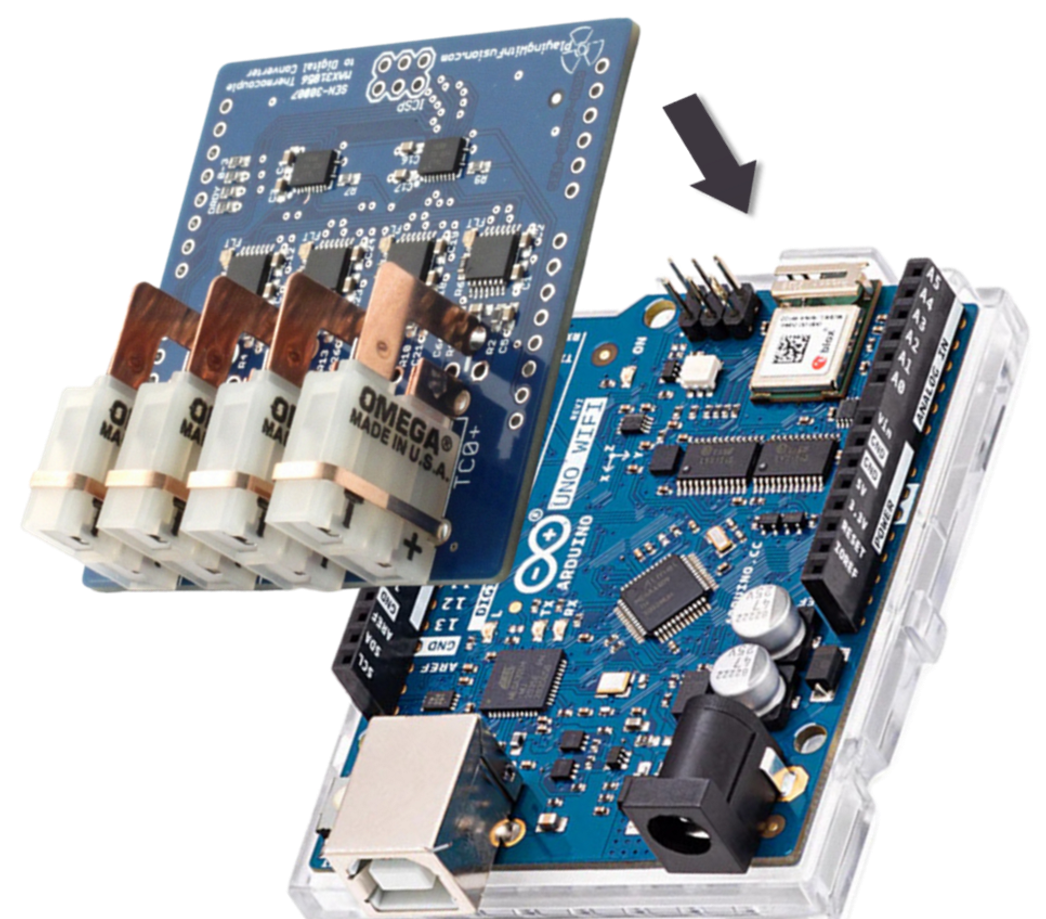
\includegraphics[width=0.7\linewidth,height=\textheight,keepaspectratio]{images/sen30007_bb.png}

}

\caption{\label{fig-MAX31856}Diagrama de conexión para el shield
MAX31856 SEN-30007.}

\end{figure}%

Acorde a PWFusion (s.~f.) sus específicaciones son las siguientes:

\begin{itemize}
\tightlist
\item
  Conversión de señal analógica a digital con resolución de 19 bits.
\item
  Interfaz ICSP de 4 hilos.
\item
  Rango de voltaje de alimentación: 3.3\,V a 5.0\,V.
\end{itemize}

Igualmente se proporciona el código de Arduino empleado:

\begin{Shaded}
\begin{Highlighting}[]
\CommentTok{\#include \textless{}PWFusion\_MAX31856.h\textgreater{}}

\OperatorTok{//}\NormalTok{ Definición de los pines chip select para cada termopar}
\NormalTok{uint8\_t tcChipSelects[] }\OperatorTok{=}\NormalTok{ \{}\DecValTok{10}\NormalTok{, }\DecValTok{9}\NormalTok{, }\DecValTok{8}\NormalTok{, }\DecValTok{7}\NormalTok{\}}\OperatorTok{;}
\CommentTok{\#define NUM\_THERMOCOUPLES   (sizeof(tcChipSelects) / sizeof(uint8\_t))}

\OperatorTok{//}\NormalTok{ Coeficientes de calibración para cada termopar}
\NormalTok{const }\BuiltInTok{float}\NormalTok{ m[NUM\_THERMOCOUPLES] }\OperatorTok{=}\NormalTok{ \{}\FloatTok{1.0450}\NormalTok{, }\FloatTok{1.0602}\NormalTok{, }\FloatTok{1.0814}\NormalTok{, }\FloatTok{1.0554}\NormalTok{\}}\OperatorTok{;}  \OperatorTok{//}\NormalTok{ Pendientes}
\NormalTok{const }\BuiltInTok{float}\NormalTok{ b[NUM\_THERMOCOUPLES] }\OperatorTok{=}\NormalTok{ \{}\OperatorTok{{-}}\FloatTok{2.4327}\NormalTok{, }\OperatorTok{{-}}\FloatTok{2.8632}\NormalTok{, }\OperatorTok{{-}}\FloatTok{4.4316}\NormalTok{, }\OperatorTok{{-}}\FloatTok{3.9348}\NormalTok{\}}\OperatorTok{;}  \OperatorTok{//}\NormalTok{ Intersecciones}

\OperatorTok{//}\NormalTok{ Se crea un objeto MAX31856 para cada termopar}
\NormalTok{MAX31856 thermocouples[NUM\_THERMOCOUPLES]}\OperatorTok{;}

\BuiltInTok{float}\OperatorTok{*}\NormalTok{ ThermocoupleTemp() \{}
\NormalTok{  static }\BuiltInTok{float}\NormalTok{ tc\_temps[NUM\_THERMOCOUPLES]}\OperatorTok{;}
\NormalTok{  static }\BuiltInTok{bool}\NormalTok{ initialized }\OperatorTok{=}\NormalTok{ false}\OperatorTok{;}

  \OperatorTok{//}\NormalTok{ Inicializa los sensores solo la primera vez que se llama a la función}
  \ControlFlowTok{if}\NormalTok{ (}\OperatorTok{!}\NormalTok{initialized) \{}
\NormalTok{    delay(}\DecValTok{1000}\NormalTok{)}\OperatorTok{;}  \OperatorTok{//}\NormalTok{ Espera para la estabilización de los sensores}
    \ControlFlowTok{for}\NormalTok{ (}\BuiltInTok{int}\NormalTok{ i }\OperatorTok{=} \DecValTok{0}\OperatorTok{;}\NormalTok{ i }\OperatorTok{\textless{}}\NormalTok{ NUM\_THERMOCOUPLES}\OperatorTok{;}\NormalTok{ i}\OperatorTok{++}\NormalTok{) \{}
\NormalTok{      thermocouples[i].begin(tcChipSelects[i])}\OperatorTok{;}
\NormalTok{      thermocouples[i].config(T\_TYPE, CUTOFF\_60HZ, AVG\_SEL\_4SAMP, CMODE\_OFF)}\OperatorTok{;}
\NormalTok{    \}}
\NormalTok{    initialized }\OperatorTok{=}\NormalTok{ true}\OperatorTok{;}
\NormalTok{  \}}
  
  \OperatorTok{//}\NormalTok{ Inicia la medición en cada sensor}
  \ControlFlowTok{for}\NormalTok{ (}\BuiltInTok{int}\NormalTok{ i }\OperatorTok{=} \DecValTok{0}\OperatorTok{;}\NormalTok{ i }\OperatorTok{\textless{}}\NormalTok{ NUM\_THERMOCOUPLES}\OperatorTok{;}\NormalTok{ i}\OperatorTok{++}\NormalTok{) \{}
\NormalTok{    thermocouples[i].startOneShotMeasurement()}\OperatorTok{;}
\NormalTok{  \}}
  
  \OperatorTok{//}\NormalTok{ Espera el tiempo necesario para que la conversión se complete}
\NormalTok{  delay(}\DecValTok{180}\NormalTok{)}\OperatorTok{;}
  
  \OperatorTok{//}\NormalTok{ Actualiza la muestra en cada sensor}
  \ControlFlowTok{for}\NormalTok{ (}\BuiltInTok{int}\NormalTok{ i }\OperatorTok{=} \DecValTok{0}\OperatorTok{;}\NormalTok{ i }\OperatorTok{\textless{}}\NormalTok{ NUM\_THERMOCOUPLES}\OperatorTok{;}\NormalTok{ i}\OperatorTok{++}\NormalTok{) \{}
\NormalTok{    thermocouples[i].sample()}\OperatorTok{;}
\NormalTok{  \}}
  
  \OperatorTok{//}\NormalTok{ Obtiene la temperatura ambiente de cada sensor y aplica la calibración}
  \ControlFlowTok{for}\NormalTok{ (}\BuiltInTok{int}\NormalTok{ i }\OperatorTok{=} \DecValTok{0}\OperatorTok{;}\NormalTok{ i }\OperatorTok{\textless{}}\NormalTok{ NUM\_THERMOCOUPLES}\OperatorTok{;}\NormalTok{ i}\OperatorTok{++}\NormalTok{) \{}
    \ControlFlowTok{if}\NormalTok{ (thermocouples[i].getStatus() }\OperatorTok{!=} \DecValTok{0}\NormalTok{) \{}
      \OperatorTok{//}\NormalTok{ En caso de error, se asigna NaN (Not a Number)}
\NormalTok{      tc\_temps[i] }\OperatorTok{=}\NormalTok{ NAN}\OperatorTok{;}
\NormalTok{    \} }\ControlFlowTok{else}\NormalTok{ \{}
      \BuiltInTok{float}\NormalTok{ raw\_temperature }\OperatorTok{=}\NormalTok{ thermocouples[i].getTemperature()}\OperatorTok{;}
\NormalTok{      tc\_temps[i] }\OperatorTok{=}\NormalTok{ m[i] }\OperatorTok{*}\NormalTok{ raw\_temperature }\OperatorTok{+}\NormalTok{ b[i]}\OperatorTok{;}  \OperatorTok{//}\NormalTok{ Aplica la calibración}
\NormalTok{    \}}
\NormalTok{  \}}
  
  \ControlFlowTok{return}\NormalTok{ tc\_temps}\OperatorTok{;}
\NormalTok{\}}
\end{Highlighting}
\end{Shaded}

\subsubsection{Fuehler Systeme TPF1/E-20
PT1000}\label{fuehler-systeme-tpf1e-20-pt1000}

Se empleó el TPF1/E-20 PT1000, diseñado para medir la temperatura
radiante en un rango de temperaturas de -30\,°C a +75\,°C. Su sonda de
temperatura, basada en la tecnología PT1000, se puede montar como un
péndulo libremente suspendido, lo que permite obtener mediciones
precisas de la temperatura de sensación térmica en entornos donde la
convección natural y la estratificación del aire pueden influir en los
resultados. FuehlerSysteme (s.~f.)

\textbf{Especificaciones}

\begin{itemize}
\tightlist
\item
  Tipo de circuito: Conexión de 2 hilos.
\item
  Corriente de medición: Aproximadamente 1\,mA.
\item
  Conexión eléctrica: Extremos pelados con terminales.
\item
  Cable: Cable de PVC (2×0,25\,mm2, temperatura máxima +105\,°C) con
  extremos de cable núcleo disponibles en diferentes longitudes.
\item
  Resistencia de fuga: Mayor a 100\,M\(\Omega\) a +20\,°C (500\,V DC).
\item
  Material del globo: Aluminio (negro).
\item
  Dimensiones del globo: Diámetro de 70\,mm.
\end{itemize}

\subsubsection{Adafruit PT1000
RTD-MAX31865}\label{adafruit-pt1000-rtd-max31865}

El PT1000 RTD-MAX31865 es un convertidor de resistencia a digital.

\begin{figure}

\centering{

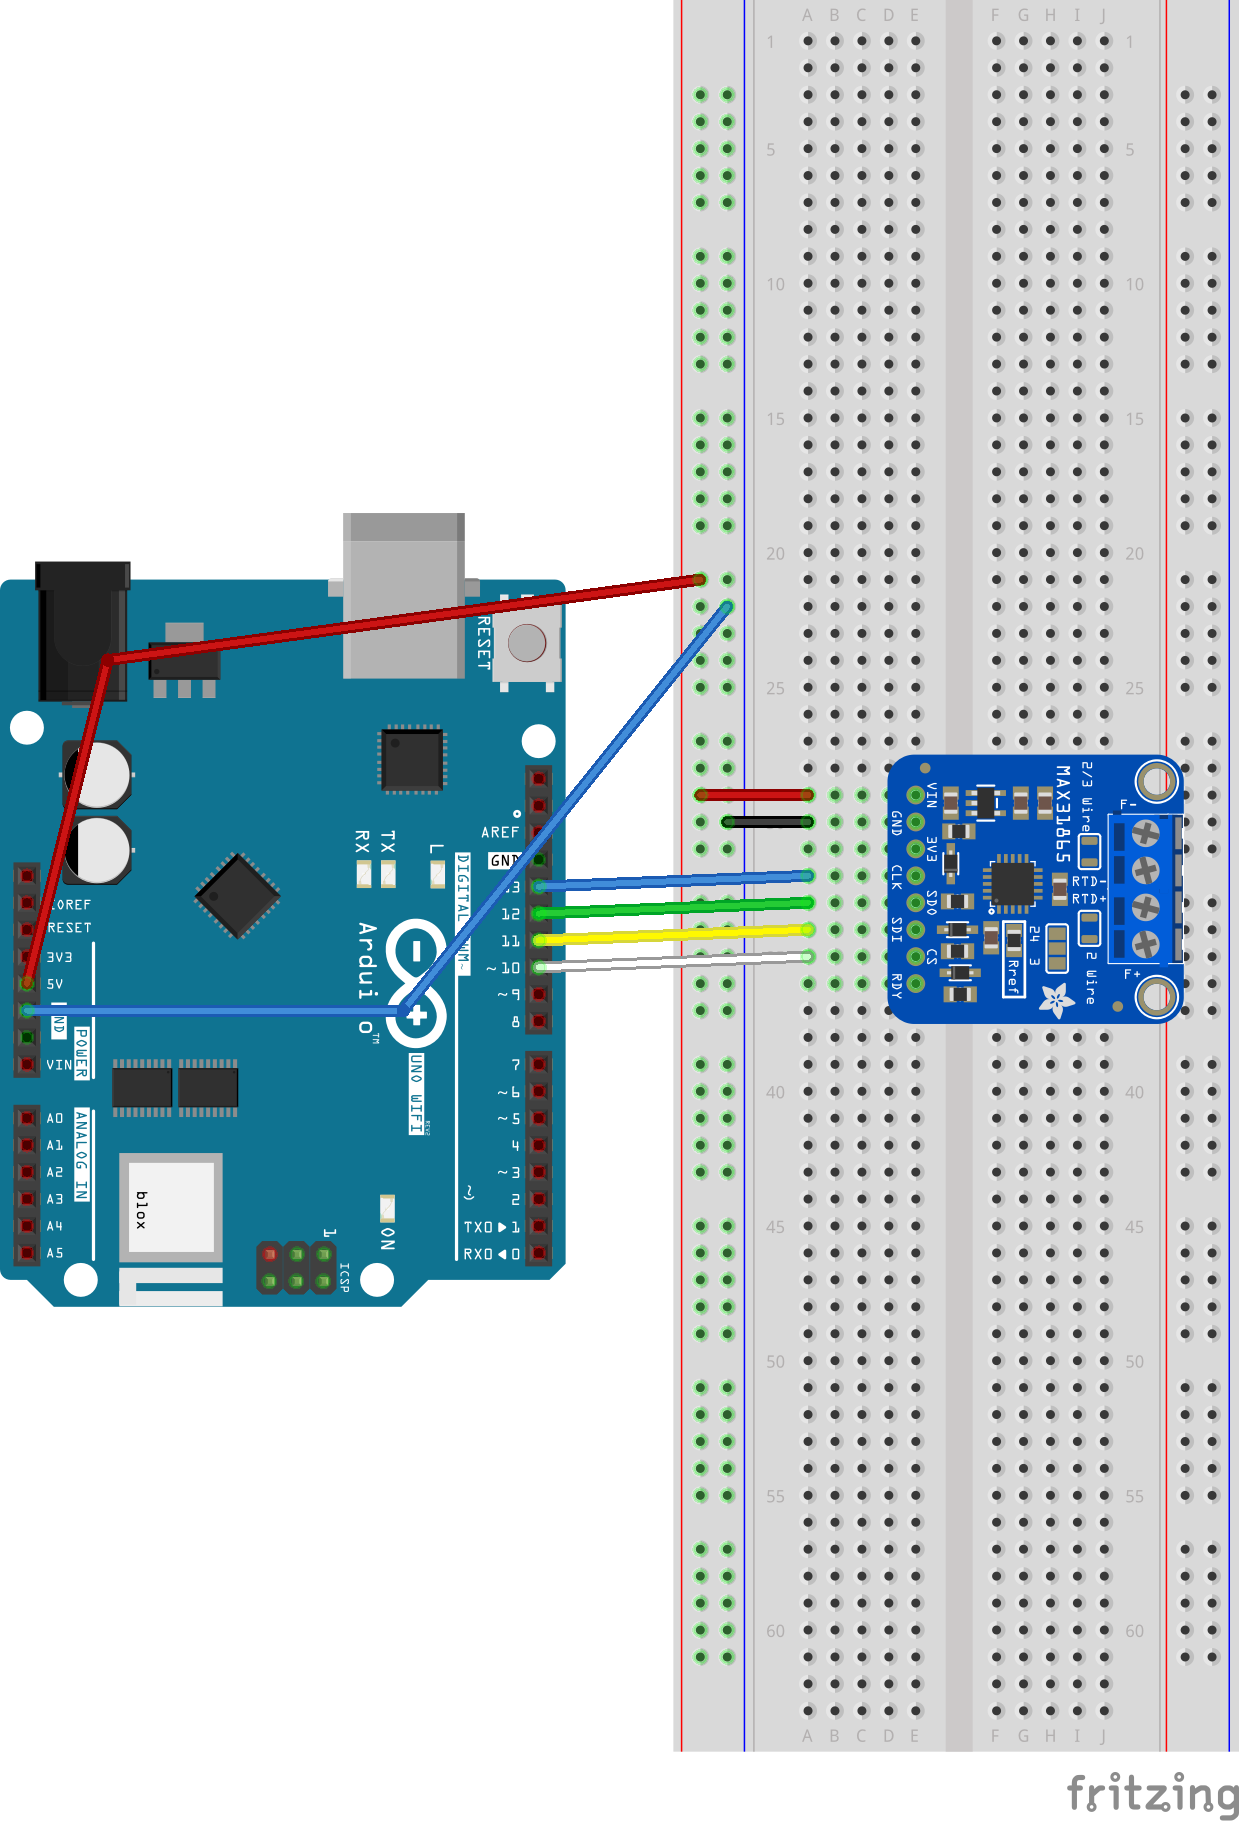
\includegraphics[width=0.7\linewidth,height=\textheight,keepaspectratio]{images/pt1000_bb.png}

}

\caption{\label{fig-MAX31865}Diagrama de conexión para el PT1000
RTD-MAX31865.}

\end{figure}%

Adafruit (s.~f.) describe las siguientes características:

\begin{itemize}
\tightlist
\item
  Realiza la conversión de la resistencia de sensores RTD de platino a
  un valor digital de forma sencilla.
\item
  Soporte con RTD de platino con valores de 100\,\(\Omega\) a
  1\,k\(\Omega\) (a 0\,°C), abarcando desde PT100 hasta PT1000.
\item
  Compatible con configuraciones de 2, 3 y 4 hilos para la conexión de
  sensores.
\item
  Incorpora una interfaz ICSP, facilitando su integración en sistemas
  basados en microcontroladores.
\item
  Cuenta con un ADC de 15 bits que proporciona una resolución nominal de
  temperatura de 0.03125\,°C (valor variable debido a la no linealidad
  del RTD) y una precisión total de hasta 0.5\,°C (0.05\% de la escala
  completa) en todas las condiciones operativas.
\item
  Tiempo máximo de conversión es de 21\,ms.
\end{itemize}

A continuación se muestra el código de Arduino:

\begin{Shaded}
\begin{Highlighting}[]
\CommentTok{\#include \textless{}Adafruit\_MAX31865.h\textgreater{}}

\OperatorTok{//}\NormalTok{ Usamos software SPI: CS, DI, DO, CLK}
\NormalTok{Adafruit\_MAX31865 thermo }\OperatorTok{=}\NormalTok{ Adafruit\_MAX31865(}\DecValTok{10}\NormalTok{, }\DecValTok{11}\NormalTok{, }\DecValTok{12}\NormalTok{, }\DecValTok{13}\NormalTok{)}\OperatorTok{;}
\OperatorTok{//}\NormalTok{ Para hardware SPI solo se pasa el pin CS}
\OperatorTok{//}\NormalTok{ Adafruit\_MAX31865 thermo }\OperatorTok{=}\NormalTok{ Adafruit\_MAX31865(}\DecValTok{10}\NormalTok{)}\OperatorTok{;}

\CommentTok{\#define RREF      4300.0  // Resistor de referencia (usa 430.0 para PT100 o 4300.0 para PT1000)}
\CommentTok{\#define RNOMINAL  1000.0  // Resistencia nominal a 0°C (100.0 para PT100, 1000.0 para PT1000)}

\OperatorTok{//}\NormalTok{ Función que realiza la medición y retorna la temperatura radiante en grados Celsius.}
\BuiltInTok{float}\NormalTok{ TPF1Temp() \{}
  \OperatorTok{//}\NormalTok{ Inicializa el sensor solo la primera vez que se llama a la función.}
\NormalTok{  static }\BuiltInTok{bool}\NormalTok{ initialized }\OperatorTok{=}\NormalTok{ false}\OperatorTok{;}
  \ControlFlowTok{if}\NormalTok{ (}\OperatorTok{!}\NormalTok{initialized) \{}
\NormalTok{    thermo.begin(MAX31865\_2WIRE)}\OperatorTok{;}  \OperatorTok{//}\NormalTok{ Inicialización }\KeywordTok{del}\NormalTok{ MAX31865}
\NormalTok{    initialized }\OperatorTok{=}\NormalTok{ true}\OperatorTok{;}
\NormalTok{  \}}
  
  \OperatorTok{//}\NormalTok{ Lectura }\KeywordTok{del}\NormalTok{ valor RTD}
\NormalTok{  uint16\_t rtd }\OperatorTok{=}\NormalTok{ thermo.readRTD()}\OperatorTok{;}
  
  \OperatorTok{//}\NormalTok{ Calcula la razón y la resistencia (opcional si se requiere para otros cálculos)}
  \BuiltInTok{float}\NormalTok{ ratio }\OperatorTok{=}\NormalTok{ rtd }\OperatorTok{/} \FloatTok{32768.0}\OperatorTok{;}
  \BuiltInTok{float}\NormalTok{ resistance }\OperatorTok{=}\NormalTok{ RREF }\OperatorTok{*}\NormalTok{ ratio}\OperatorTok{;}
  
  \OperatorTok{//}\NormalTok{ Calcula la temperatura utilizando el método de la librería}
  \BuiltInTok{float}\NormalTok{ raw\_temp }\OperatorTok{=}\NormalTok{ thermo.temperature(RNOMINAL, RREF)}\OperatorTok{;}

  \OperatorTok{//}\NormalTok{ Aplica la ecuación de calibración: }\FloatTok{1.0582} \OperatorTok{*}\NormalTok{ temp }\OperatorTok{+}\NormalTok{ (}\OperatorTok{{-}}\FloatTok{1.5553}\NormalTok{)}
  \BuiltInTok{float}\NormalTok{ radiant\_temp }\OperatorTok{=} \FloatTok{1.0582} \OperatorTok{*}\NormalTok{ raw\_temp }\OperatorTok{{-}} \FloatTok{1.5553}\OperatorTok{;}
  
  \ControlFlowTok{return}\NormalTok{ radiant\_temp}\OperatorTok{;}
\NormalTok{\}}
\end{Highlighting}
\end{Shaded}

\subsubsection{Modern Device Wind Sensor
Rev.~P6}\label{modern-device-wind-sensor-rev.-p6}

El sensor de viento Rev.~P6 es un anemómetro de hilo caliente. Incorpora
un potenciómetro de alta precisión para facilitar la calibración
(realizada en fábrica) y utilizar termistores de coeficiente de
temperatura positivo, que aseguran mediciones más estables incluso ante
variaciones de temperatura ambiente. Requiere una fuente de alimentación
de 9 a 12\,V (idealmente 12\,V) para garantizar el adecuado
calentamiento de los termistores y evitar la saturación en condiciones
de viento intenso. Integra un sensor de temperatura ambiental con salida
escalada a 3.3\,V y una señal de viento ajustada a un máximo de 3.3\,V
mediante resistencias de alta precisión. ModernDevice (s.~f.)

\begin{figure}

\centering{

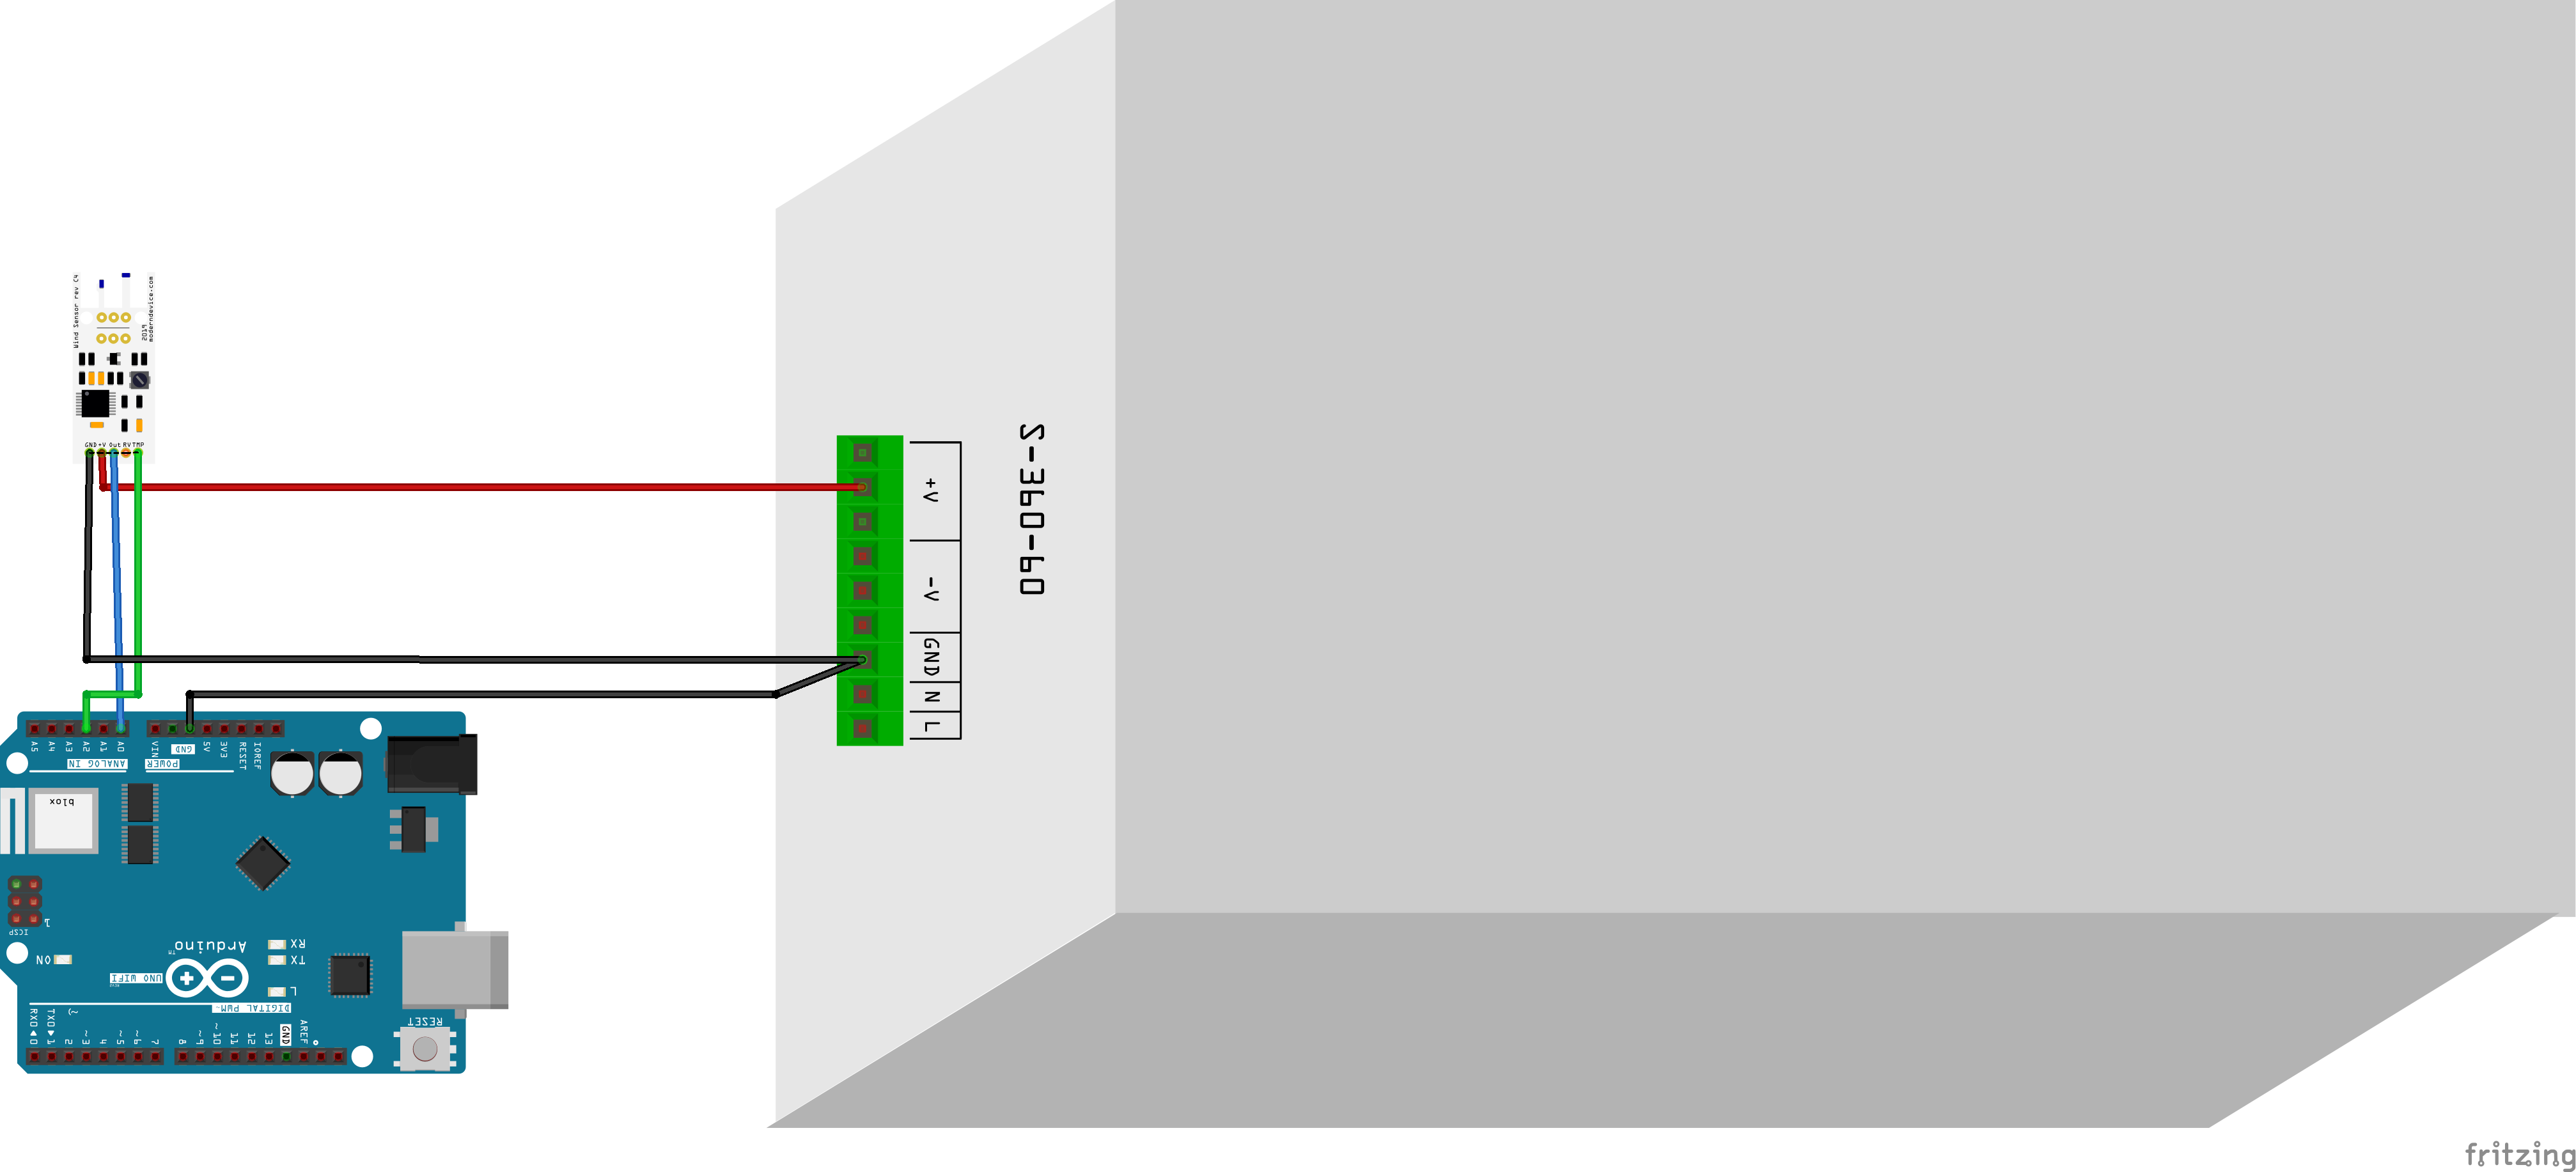
\includegraphics[width=0.7\linewidth,height=\textheight,keepaspectratio]{images/windsensor_bb.png}

}

\caption{\label{fig-WindSensor}Diagrama de conexión para el Wind Sensor
Rev.~P6.}

\end{figure}%

\textbf{Especificaciones}

\begin{itemize}
\tightlist
\item
  Voltaje de alimentación: 10--12\,V.
\item
  Corriente: Aproximadamente 40\,mA.
\item
  Velocidades de viento medidas: 0--150\,mph.
\item
  Compensación de temperatura ambiente.
\end{itemize}

\begin{Shaded}
\begin{Highlighting}[]
\CommentTok{\#include \textless{}math.h\textgreater{}}

\NormalTok{const }\BuiltInTok{int}\NormalTok{ OutPin  }\OperatorTok{=}\NormalTok{ A0}\OperatorTok{;}   \OperatorTok{//}\NormalTok{ Pin analógico para el sensor de viento (}\StringTok{"OUT"}\NormalTok{)}
\NormalTok{const }\BuiltInTok{int}\NormalTok{ TempPin }\OperatorTok{=}\NormalTok{ A2}\OperatorTok{;}   \OperatorTok{//}\NormalTok{ Pin analógico para el sensor de temperatura (}\StringTok{"TMP"}\NormalTok{)}

\OperatorTok{//}\NormalTok{ Función que lee velocidad de viento y temperatura, y retorna un array de dos floats:}
\OperatorTok{//}\NormalTok{ ws[}\DecValTok{0}\NormalTok{] }\OperatorTok{{-}\textgreater{}}\NormalTok{ velocidad de viento (m}\OperatorTok{/}\NormalTok{s)}
\OperatorTok{//}\NormalTok{ ws[}\DecValTok{1}\NormalTok{] }\OperatorTok{{-}\textgreater{}}\NormalTok{ temperatura (°C)}
\BuiltInTok{float}\OperatorTok{*}\NormalTok{ WindSensor() \{}
\NormalTok{  static }\BuiltInTok{float}\NormalTok{ ws[}\DecValTok{2}\NormalTok{]}\OperatorTok{;}
  
  \OperatorTok{//}\NormalTok{ Lectura }\KeywordTok{del}\NormalTok{ sensor de viento}
  \BuiltInTok{int}\NormalTok{ windADunits }\OperatorTok{=}\NormalTok{ analogRead(OutPin)}\OperatorTok{;}
  \BuiltInTok{float}\NormalTok{ voltage }\OperatorTok{=}\NormalTok{ (}\BuiltInTok{float}\NormalTok{)windADunits }\OperatorTok{*} \FloatTok{5.0} \OperatorTok{/} \FloatTok{1024.0}\OperatorTok{;}
  
  \OperatorTok{//}\NormalTok{ Aplicar la corrección al voltaje}
  \BuiltInTok{float}\NormalTok{ correctedVoltage }\OperatorTok{=}\NormalTok{ voltage }\OperatorTok{{-}} \FloatTok{1.1621}\OperatorTok{;}
  
  \OperatorTok{//}\NormalTok{ Lectura }\KeywordTok{del}\NormalTok{ sensor de temperatura}
  \BuiltInTok{int}\NormalTok{ tempRawAD }\OperatorTok{=}\NormalTok{ analogRead(TempPin)}\OperatorTok{;}
  \BuiltInTok{float}\NormalTok{ tempC }\OperatorTok{=}\NormalTok{ ((((}\BuiltInTok{float}\NormalTok{)tempRawAD }\OperatorTok{*} \FloatTok{5.0}\NormalTok{) }\OperatorTok{/} \FloatTok{1024.0}\NormalTok{) }\OperatorTok{{-}} \FloatTok{0.400}\NormalTok{) }\OperatorTok{/} \FloatTok{0.0195}\OperatorTok{;}
  
  \OperatorTok{//}\NormalTok{ Cálculo de la velocidad de viento en m}\OperatorTok{/}\NormalTok{s usando la ecuación empírica:}
  \OperatorTok{//}\NormalTok{ WS }\OperatorTok{=} \FloatTok{26.3431} \OperatorTok{*}\NormalTok{ (correctedVoltage)}\OperatorTok{\^{}}\NormalTok{(}\FloatTok{1.4273}\NormalTok{) }\OperatorTok{*}\NormalTok{ (tempC)}\OperatorTok{\^{}}\NormalTok{(}\OperatorTok{{-}}\FloatTok{0.7631}\NormalTok{)}
  \BuiltInTok{float}\NormalTok{ windSpeed }\OperatorTok{=} \FloatTok{26.3431} \OperatorTok{*} \BuiltInTok{pow}\NormalTok{(correctedVoltage, }\FloatTok{1.4273}\NormalTok{) }\OperatorTok{*} \BuiltInTok{pow}\NormalTok{(tempC, }\OperatorTok{{-}}\FloatTok{0.7631}\NormalTok{)}\OperatorTok{;}
  
\NormalTok{  ws[}\DecValTok{0}\NormalTok{] }\OperatorTok{=}\NormalTok{ windSpeed}\OperatorTok{;}
\NormalTok{  ws[}\DecValTok{1}\NormalTok{] }\OperatorTok{=}\NormalTok{ tempC}\OperatorTok{;}
  
  \ControlFlowTok{return}\NormalTok{ ws}\OperatorTok{;}
\NormalTok{\}}
\end{Highlighting}
\end{Shaded}

\subsection{Raspberry Pi 4 Model B}\label{raspberry-pi-4-model-b}

El Raspberry Pi 4 Model B es una computadora de placa única de alto
rendimiento, diseñada para tareas de procesamiento avanzado y
conectividad eficiente en un formato compacto. Equipada con un
procesador de 64 bits de cuatro núcleos y opciones de RAM de hasta 8 GB,
ofrece soporte para salida de video dual 4K y conectividad avanzada
mediante Wi-Fi de doble banda, Bluetooth 5.0, Ethernet Gigabit y puertos
USB 3.0, con capacidad para Power over Ethernet (PoE) mediante un
accesorio adicional. Su diseño versátil y eficiente la hace ideal para
la integración y gestión de datos en el sistema DTHIS-C. Raspberry
(2019)

En la Tabla~\ref{tbl-raspberry} se muestran sus especificaciones.

\begin{longtable}[]{@{}
  >{\raggedright\arraybackslash}p{(\linewidth - 2\tabcolsep) * \real{0.3636}}
  >{\raggedright\arraybackslash}p{(\linewidth - 2\tabcolsep) * \real{0.6364}}@{}}
\caption{Especificaciones del Raspberry Pi 4 Model
B.}\label{tbl-raspberry}\tabularnewline
\toprule\noalign{}
\begin{minipage}[b]{\linewidth}\raggedright
\textbf{Parámetro}
\end{minipage} & \begin{minipage}[b]{\linewidth}\raggedright
\textbf{Detalle}
\end{minipage} \\
\midrule\noalign{}
\endfirsthead
\toprule\noalign{}
\begin{minipage}[b]{\linewidth}\raggedright
\textbf{Parámetro}
\end{minipage} & \begin{minipage}[b]{\linewidth}\raggedright
\textbf{Detalle}
\end{minipage} \\
\midrule\noalign{}
\endhead
\bottomrule\noalign{}
\endlastfoot
Procesador & Broadcom BCM2711, 4 núcleos Cortex-A72, 1.5 GHz \\
Memoria RAM & 8 GB (LPDDR4-3200) \\
Conectividad Wi-Fi & Sí, dual-band 2.4 GHz y 5 GHz, 802.11ac \\
Bluetooth & Sí, Bluetooth 5.0 \\
Puertos USB & 2 USB 3.0, 2 USB 2.0 \\
Salida de video & 2 micro HDMI, soporte dual 4K 60 fps \\
Ethernet & Gigabit \\
Almacenamiento & Tarjeta microSD \\
Voltaje de operación & 5V \\
Consumo energético & Eficiente, sin ventilador (\textasciitilde3A
recomendado) \\
Dimensiones & 85.6 mm x 56.5 mm x 17 mm \\
\end{longtable}

El siguiente código constituye el programa principal del Raspberry Pi 4
Model B en el DTHIS-C, encargado de gestionar la conexión al servidor
ThingsBoard mediante el protocolo MQTT y el envío de datos provenientes
de sensores como el SCD30 (CO2, temperatura y humedad relativa). Escrito
en Python, utiliza la librería \texttt{paho-mqtt} para la comunicación y
está diseñado para operar de manera continua:

\begin{Shaded}
\begin{Highlighting}[]
\ImportTok{import}\NormalTok{ paho.mqtt.client }\ImportTok{as}\NormalTok{ mqtt}
\ImportTok{import}\NormalTok{ json}
\ImportTok{import}\NormalTok{ time}
\ImportTok{from}\NormalTok{ thingsboard\_credentials }\ImportTok{import}\NormalTok{ thingsboard\_data}
\ImportTok{from}\NormalTok{ scd30 }\ImportTok{import}\NormalTok{ scd30\_measurements}
\ImportTok{from}\NormalTok{ sound }\ImportTok{import}\NormalTok{ sound\_data}

\CommentTok{\# Obtiene los datos de conexión para ThingsBoard}
\NormalTok{unique\_id, token, thingsboard\_host }\OperatorTok{=}\NormalTok{ thingsboard\_data()}

\CommentTok{\# Diccionario para almacenar las lecturas del sensor}
\NormalTok{sensor\_data }\OperatorTok{=}\NormalTok{ \{}\StringTok{\textquotesingle{}CO2\textquotesingle{}}\NormalTok{: }\DecValTok{0}\NormalTok{, }\StringTok{\textquotesingle{}T\textquotesingle{}}\NormalTok{: }\DecValTok{0}\NormalTok{, }\StringTok{\textquotesingle{}HR\textquotesingle{}}\NormalTok{: }\DecValTok{0}\NormalTok{\}}
\CommentTok{\# Diccionario para datos de sonido}
\CommentTok{\# micro\_data = \{\textquotesingle{}RMS\textquotesingle{}: 0, \textquotesingle{}dBmax\textquotesingle{}: 0, \textquotesingle{}dBmin\textquotesingle{}: 0\}  }

\CommentTok{\# Configura el cliente MQTT}
\NormalTok{client }\OperatorTok{=}\NormalTok{ mqtt.Client(unique\_id, }\VariableTok{False}\NormalTok{)}
\NormalTok{client.username\_pw\_set(token, password}\OperatorTok{=}\VariableTok{None}\NormalTok{)}
\NormalTok{client.}\ExtensionTok{connect}\NormalTok{(thingsboard\_host, }\DecValTok{1883}\NormalTok{, }\DecValTok{60}\NormalTok{, }\StringTok{\textquotesingle{}\textquotesingle{}}\NormalTok{)}
\NormalTok{client.loop\_start()}

\ControlFlowTok{try}\NormalTok{:}
    \ControlFlowTok{while} \VariableTok{True}\NormalTok{:}
        \CommentTok{\# Obtiene las mediciones del sensor SCD30}
\NormalTok{        CO2, T, HR }\OperatorTok{=}\NormalTok{ scd30\_measurements()}

        \CommentTok{\# Actualiza el diccionario con las lecturas actuales}
\NormalTok{        sensor\_data[}\StringTok{\textquotesingle{}CO2\textquotesingle{}}\NormalTok{] }\OperatorTok{=}\NormalTok{ CO2}
\NormalTok{        sensor\_data[}\StringTok{\textquotesingle{}T\textquotesingle{}}\NormalTok{] }\OperatorTok{=}\NormalTok{ T}
\NormalTok{        sensor\_data[}\StringTok{\textquotesingle{}HR\textquotesingle{}}\NormalTok{] }\OperatorTok{=}\NormalTok{ HR}

        \CommentTok{\# Publica los datos del SCD30 en ThingsBoard}
\NormalTok{        client.publish(}\StringTok{\textquotesingle{}v1/devices/me/telemetry\textquotesingle{}}\NormalTok{, json.dumps(sensor\_data), }\DecValTok{1}\NormalTok{)}

        \CommentTok{\# Obtiene los datos de sonido}
        \CommentTok{\# micro\_data = sound\_data() }

        \CommentTok{\# Publica los datos de sonido en ThingsBoard}
        \CommentTok{\# client.publish(\textquotesingle{}v1/devices/me/telemetry\textquotesingle{}, json.dumps(micro\_data), 1)}

\NormalTok{        time.sleep(}\DecValTok{2}\NormalTok{)  }\CommentTok{\# Ajusta el intervalo de tiempo entre lecturas}

\ControlFlowTok{except} \PreprocessorTok{KeyboardInterrupt}\NormalTok{:}
    \ControlFlowTok{pass}

\CommentTok{\# Detiene el loop del cliente MQTT y desconecta del servidor}
\NormalTok{client.loop\_stop()}
\NormalTok{client.disconnect()}
\end{Highlighting}
\end{Shaded}

\subsubsection{Sensirion SCD30}\label{sensirion-scd30}

El SCD30 es un sensor de CO2 basado en tecnología de detección por
infrarrojos. Incorpora un sensor de humedad y temperatura. Cuenta con un
diseño de doble canal. Además, ofrece una precisión de ±(30 ppm + 3\% de
la lectura) en un rango de 400 a 10,000 ppm. Sensirion (s.~f.)

\begin{figure}

\centering{

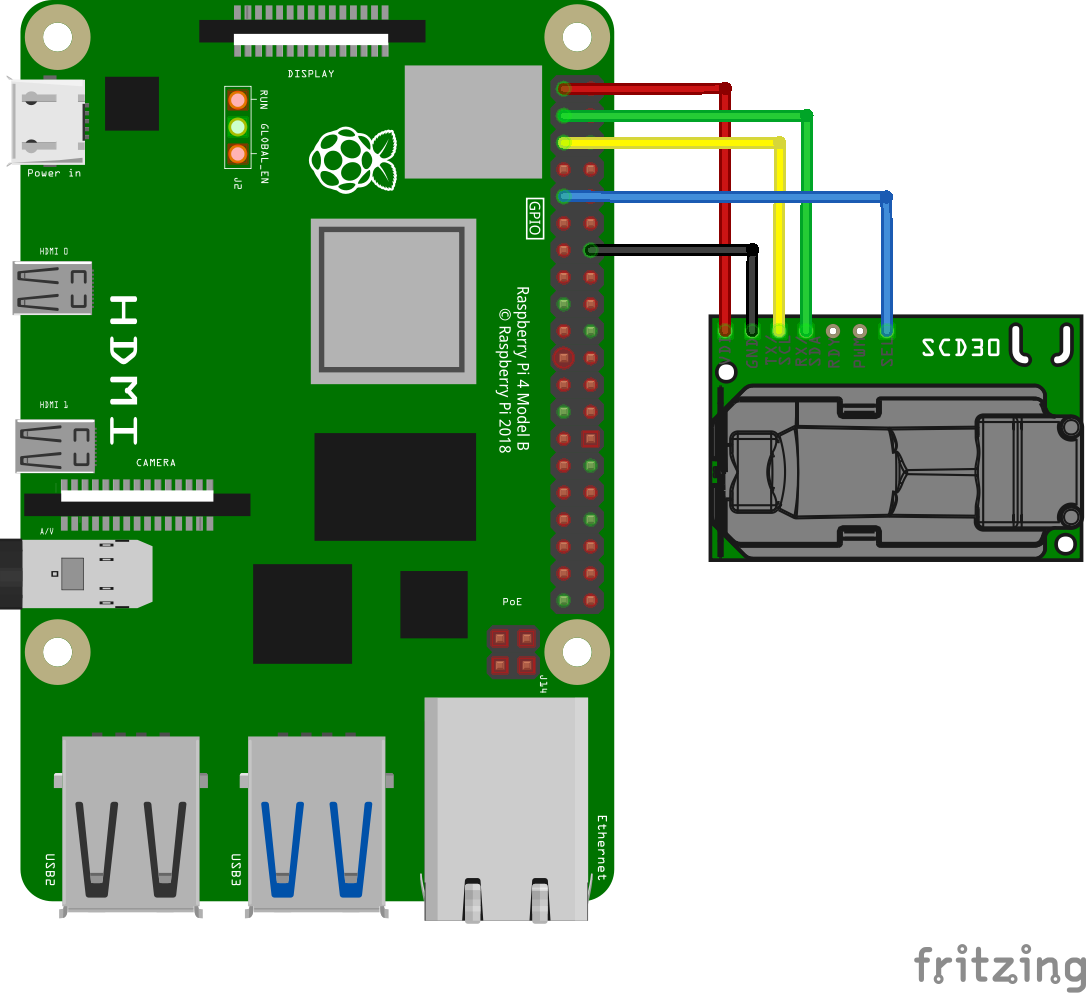
\includegraphics[width=0.7\linewidth,height=\textheight,keepaspectratio]{images/scd30_bb.png}

}

\caption{\label{fig-SCD30}Diagrama de conexión para el SCD30.}

\end{figure}%

\textbf{Especificaciones}

\textbf{CO2}

\begin{itemize}
\tightlist
\item
  Rango de medición: 400 -- 10,000 ppm
\item
  Precisión: ±30 ppm ±3\% del valor medido
\item
  Tiempo de respuesta (τ63\%): 20 s
\item
  Estabilidad térmica: 2.5 ppm/°C
\end{itemize}

\textbf{Humedad}

\begin{itemize}
\tightlist
\item
  Precisión típica: ±3 \%RH
\item
  Rango de operación: 0 -- 95 \%RH
\item
  Tiempo de respuesta (τ63\%): 8 s
\item
  Certificación de calibración: Calibrado de fábrica
\item
  Temperatura
\item
  Precisión típica: ±0.4 °C
\item
  Tiempo de respuesta (τ63\%): 10 s
\end{itemize}

\textbf{Características generales}

\begin{itemize}
\tightlist
\item
  Voltaje de alimentación: 3.3 -- 5.5 V
\item
  Corriente promedio: 19 mA
\item
  Corriente máxima: 75 mA
\item
  Rango de temperatura de operación: 0 -- 50 °C
\item
  Interfaces: I²C, ModBus, PWM
\item
  Dimensiones: 35 × 23 × 7 mm
\end{itemize}

A continuación se muestra el código de Python empleado para su
incorpación al DTHIS-C:

\begin{Shaded}
\begin{Highlighting}[]
\ImportTok{import}\NormalTok{ time}
\ImportTok{import}\NormalTok{ board}
\ImportTok{import}\NormalTok{ busio}
\ImportTok{from}\NormalTok{ scd30\_i2c }\ImportTok{import}\NormalTok{ SCD30}

\KeywordTok{def}\NormalTok{ scd30\_measurements():}
    \CommentTok{"""}
\CommentTok{    Función para obtener las lecturas de CO2, Temperatura y Humedad Relativa del sensor SCD30.}

\CommentTok{    Retorna:}
\CommentTok{        tuple: (CO2, T, HR) donde}
\CommentTok{            CO2: concentración de CO2 en ppm}
\CommentTok{            T: temperatura en grados Celsius}
\CommentTok{            HR: humedad relativa en porcentaje}
\CommentTok{    """}
    \CommentTok{\# Inicializa el sensor SCD30}
\NormalTok{    scd30 }\OperatorTok{=}\NormalTok{ SCD30()}
    \CommentTok{\# Espera para asegurarse de que el sensor esté listo}
\NormalTok{    time.sleep(}\DecValTok{2}\NormalTok{)  }
    
    \CommentTok{\# Verifica si los datos están listos para ser leídos}
    \ControlFlowTok{if}\NormalTok{ scd30.get\_data\_ready():}
        \CommentTok{\# Lee las mediciones del sensor}
\NormalTok{        CO2, T, HR }\OperatorTok{=}\NormalTok{ scd30.read\_measurement()}
        \CommentTok{\# Redondea cada valor a dos decimales}
\NormalTok{        CO2 }\OperatorTok{=} \BuiltInTok{round}\NormalTok{(CO2, }\DecValTok{2}\NormalTok{)}
\NormalTok{        T }\OperatorTok{=} \BuiltInTok{round}\NormalTok{(T, }\DecValTok{2}\NormalTok{)}
\NormalTok{        HR }\OperatorTok{=} \BuiltInTok{round}\NormalTok{(HR, }\DecValTok{2}\NormalTok{)}
        \ControlFlowTok{return}\NormalTok{ CO2, T, HR}
\end{Highlighting}
\end{Shaded}

\subsubsection{Arducam 5MP OV5647 Ultra Wide
Angle}\label{arducam-5mp-ov5647-ultra-wide-angle}

La cámara Arducam Ultra Wide Angle cuenta con un objetivo ojo de pez M12
que ofrece un campo de visión horizontal de 220°. Arducam (s.~f.)

\begin{figure}

\centering{

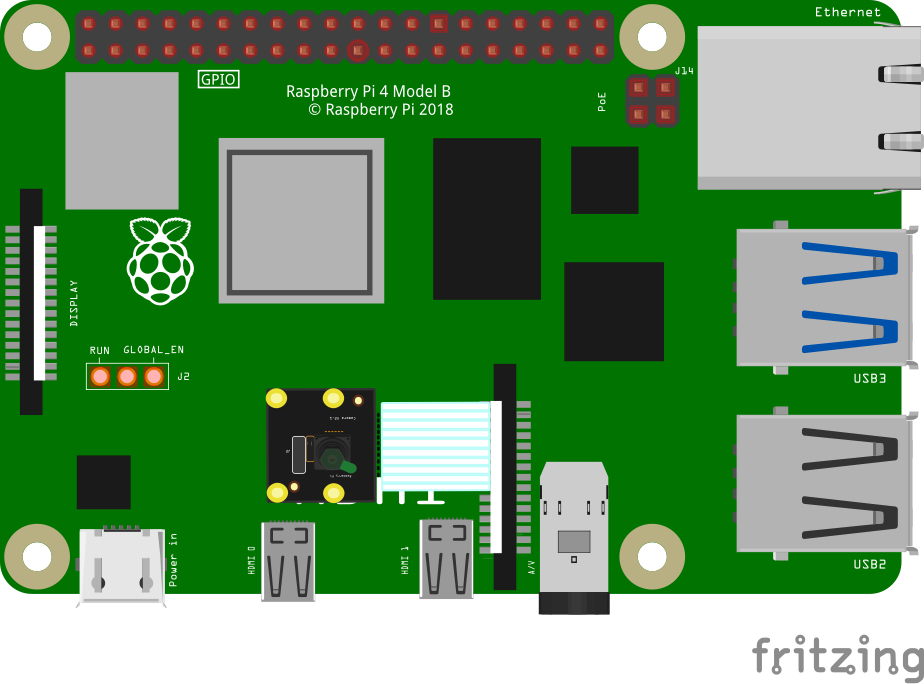
\includegraphics[width=0.7\linewidth,height=\textheight,keepaspectratio]{images/camera_bb.png}

}

\caption{\label{fig-Camara}Diagrama de conexión para la cámara OV5647.}

\end{figure}%

\textbf{Especificaciones}

\begin{itemize}
\tightlist
\item
  Sensor: Omnivision OV5647
\item
  Tamaño del sensor: 1/4″ (OV5647)
\item
  Resolución: 5 MP (2592×1944)
\item
  Video:

  \begin{itemize}
  \tightlist
  \item
    1080p a 30 fps
  \item
    720p a 60 fps
  \item
    480p a 90 fps
  \end{itemize}
\item
  Sensibilidad IR: Filtro IR-cut integrado (solo luz visible)
\item
  Campo de visión horizontal (HFOV): 220°
\item
  Distancia focal efectiva: 0.76 mm
\item
  Distancia focal equivalente en 35 mm: 8.2 mm
\item
  Tipo de enfoque: Manual
\item
  Montura del objetivo: M12
\item
  Dimensiones: 36 mm × 36 mm
\item
  Corriente pico: 300 mA
\end{itemize}

A continuación, se muestra el código escrito en Bash/Shell que accede a
la cámara y, posteriormente, genera los mapas de luminancia:

\begin{Shaded}
\begin{Highlighting}[]
\CommentTok{\#!/bin/bash}

\NormalTok{DATE}\OperatorTok{=}\NormalTok{$(date }\OperatorTok{+}\StringTok{"\%Y{-}\%m{-}}\SpecialCharTok{\%d}\StringTok{\_\%H\%M"}\NormalTok{)}
\NormalTok{IMG\_DIR}\OperatorTok{=}\StringTok{"/home/hdeza/Luminance/images"}
\NormalTok{HDR\_IMG}\OperatorTok{=}\StringTok{"/home/hdeza/Luminance/HDR\_images"}
\NormalTok{MAPS\_DIR}\OperatorTok{=}\StringTok{"/home/hdeza/Luminance/maps"}
\NormalTok{OUTPUT\_DIR}\OperatorTok{=}\StringTok{"/home/hdeza/Luminance"}

\CommentTok{\#Loop through shutter speeds and capture images}
\NormalTok{SHUTTERS}\OperatorTok{=}\NormalTok{(}\DecValTok{100} \DecValTok{500} \DecValTok{1000} \DecValTok{5000} \DecValTok{10000} \DecValTok{50000} \DecValTok{100000} \DecValTok{500000} \DecValTok{1000000} \DecValTok{2000000}\NormalTok{)}

\ControlFlowTok{for}\NormalTok{ i }\KeywordTok{in} \StringTok{"$\{!SHUTTERS[@]\}"}\OperatorTok{;}\NormalTok{ do}
\NormalTok{  rpicam}\OperatorTok{{-}}\NormalTok{still }\OperatorTok{{-}{-}}\NormalTok{raw }\OperatorTok{{-}}\NormalTok{n }\OperatorTok{{-}{-}}\NormalTok{gain }\DecValTok{1} \OperatorTok{{-}}\NormalTok{t }\DecValTok{500} \OperatorTok{{-}{-}}\NormalTok{shutter }\StringTok{"$}\SpecialCharTok{\{SHUTTERS[$i]\}}\StringTok{"} \OperatorTok{{-}}\NormalTok{o }\StringTok{"$IMG\_DIR/$(printf "}\OperatorTok{\%}\DecValTok{0}\ErrorTok{2d}\StringTok{" $((i+1))).jpg"}
\NormalTok{done}

\CommentTok{\#Run raw2hdr with the path to the images and save as image.hdr}
\NormalTok{raw2hdr }\OperatorTok{{-}}\NormalTok{a }\OperatorTok{{-}}\NormalTok{e }\OperatorTok{{-}}\NormalTok{g }\OperatorTok{{-}}\NormalTok{f }\OperatorTok{{-}}\NormalTok{h }\OperatorTok{{-}}\NormalTok{w }\OperatorTok{{-}}\NormalTok{o }\StringTok{"$HDR\_IMG/image\_$DATE.hdr"} \StringTok{"$IMG\_DIR"}\OperatorTok{/*}\NormalTok{dng}

\CommentTok{\#Get info about the final HDR}
\NormalTok{getinfo }\StringTok{"$HDR\_IMG/image\_$DATE.hdr"}

\CommentTok{\#Nullify exposure value}
\NormalTok{ra\_xyze }\OperatorTok{{-}}\NormalTok{r }\OperatorTok{{-}}\NormalTok{o }\StringTok{"$HDR\_IMG/image\_$DATE.hdr"} \OperatorTok{\textgreater{}} \StringTok{"$OUTPUT\_DIR/image\_nullEV\_$DATE.hdr"}

\CommentTok{\#Resize image}
\NormalTok{pfilt }\OperatorTok{{-}}\DecValTok{1} \OperatorTok{{-}}\NormalTok{x }\DecValTok{1000} \OperatorTok{{-}}\NormalTok{y }\DecValTok{1000} \StringTok{"$OUTPUT\_DIR/image\_nullEV\_$DATE.hdr"} \OperatorTok{\textgreater{}} \StringTok{"$OUTPUT\_DIR/image\_resize\_$DATE.hdr"}

\CommentTok{\#Make photometric adjustment}
\NormalTok{pcomb }\OperatorTok{{-}}\NormalTok{s }\FloatTok{1.8} \StringTok{"$OUTPUT\_DIR/image\_resize\_$DATE.hdr"} \OperatorTok{\textgreater{}} \StringTok{"$OUTPUT\_DIR/image\_photometric\_$DATE.hdr"}

\CommentTok{\#Change view angle for fisheye}
\NormalTok{getinfo }\OperatorTok{{-}}\NormalTok{a }\StringTok{"VIEW= {-}vta {-}vv 160 {-}vh 160"} \OperatorTok{\textless{}} \StringTok{"$OUTPUT\_DIR/image\_photometric\_$DATE.hdr"} \OperatorTok{\textgreater{}} \StringTok{"$IMG\_DIR/image\_final\_$DATE.hdr"}

\CommentTok{\#Print illuminance value}
\NormalTok{echo }\StringTok{"Total illuminance is: "}
\NormalTok{evalglare }\OperatorTok{{-}}\NormalTok{V }\StringTok{"$IMG\_DIR/image\_final\_$DATE.hdr"}
\NormalTok{evalglare }\OperatorTok{{-}}\NormalTok{V }\StringTok{"$IMG\_DIR/image\_final\_$DATE.hdr"} \OperatorTok{\textgreater{}} \StringTok{"$OUTPUT\_DIR/illuminance\_$DATE.txt"}

\CommentTok{\#Move final HDR image to HDR\_images}
\NormalTok{mv }\StringTok{"$IMG\_DIR/image\_final\_$DATE.hdr"} \StringTok{"$HDR\_IMG/image\_final\_$DATE.hdr"}

\CommentTok{\#Crop to a 160}
\NormalTok{pcomb }\OperatorTok{{-}}\NormalTok{e }\StringTok{\textquotesingle{}Cx:xmax/2;Cy:ymax/2;R:444.44;sq(x):x*x\textquotesingle{}} \OperatorTok{{-}}\NormalTok{e }\StringTok{\textquotesingle{}inC=sq(R){-}sq(x{-}Cx){-}sq(y{-}Cy)\textquotesingle{}} \OperatorTok{{-}}\NormalTok{e }\StringTok{\textquotesingle{}ro=if(inC,ri(1),0);go=if(inC,gi(1),0);bo=if(inC,bi(1),0)\textquotesingle{}} \StringTok{"$HDR\_IMG/image\_final\_$DATE.hdr"} \OperatorTok{\textgreater{}} \StringTok{"$HDR\_IMG/image\_crop\_$DATE.hdr"}

\CommentTok{\#Make the luminance map with configurations and save it}
\NormalTok{falsecolor }\OperatorTok{{-}}\NormalTok{s }\DecValTok{5000} \OperatorTok{{-}}\NormalTok{d }\DecValTok{1} \OperatorTok{{-}}\NormalTok{i }\StringTok{"$HDR\_IMG/image\_crop\_$DATE.hdr"} \OperatorTok{{-}{-}}\NormalTok{log }\DecValTok{3} \OperatorTok{\textgreater{}} \StringTok{"$MAPS\_DIR/image\_map\_$DATE.hdr"}
\end{Highlighting}
\end{Shaded}

\subsubsection{Micrófono ambiental
USB}\label{micruxf3fono-ambiental-usb}

El micrófono incorpora un filtro que atenúa eficazmente los ruidos
producidos por el viento o la respiración. Su patrón de captación
direccional optimiza la focalización de la fuente sonora. Steren (s.~f.)

\begin{figure}

\centering{

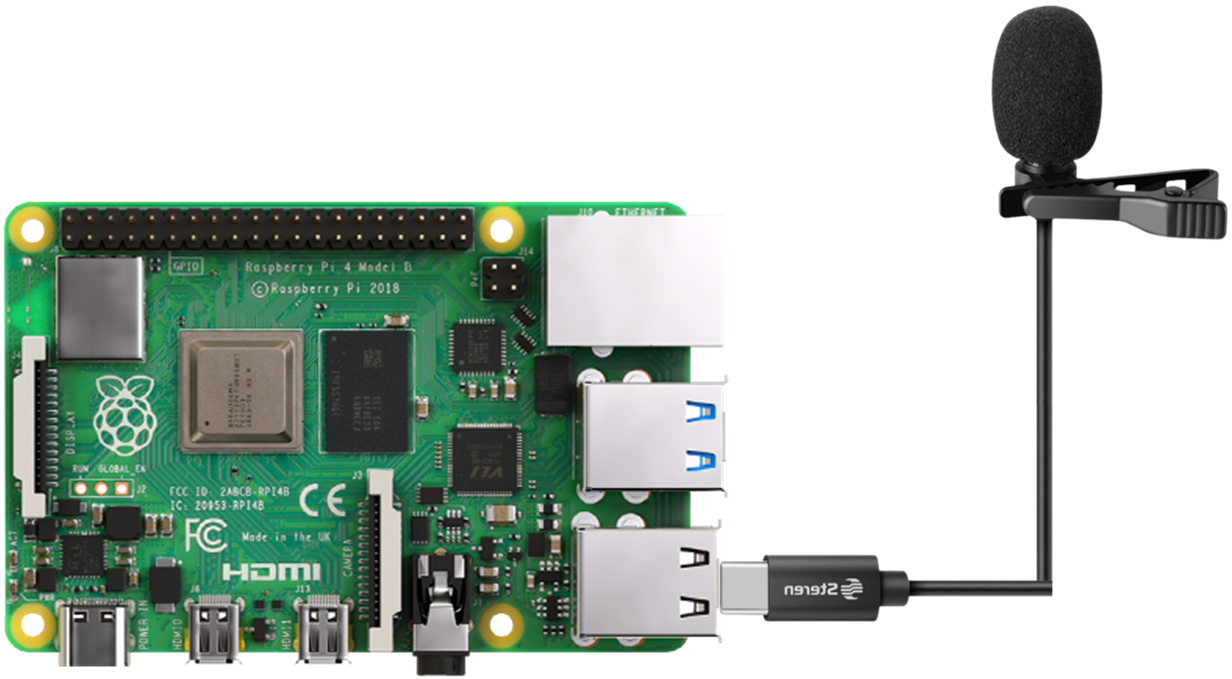
\includegraphics[width=0.7\linewidth,height=\textheight,keepaspectratio]{images/micro_bb.png}

}

\caption{\label{fig-Microfono}Diagrama de conexión para el micrófono.}

\end{figure}%

\textbf{Especificaciones}

\begin{itemize}
\tightlist
\item
  Respuesta en frecuencia: 50 a 10,000 Hz
\item
  Impedancia 2,200 \(\Omega\)
\item
  Sensibilidad: -32 dB ±3 dB
\end{itemize}

A continuación, se presentan los códigos utilizados para la captura y
análisis de sonido. Estos scripts permiten grabar el audio, extraer
parámetros clave de la señal y convertirlos a valores en decibeles (dB).

El siguiente script graba un archivo de audio en formato WAV durante 15
segundos a una frecuencia de muestreo de 44.1 kHz:

\begin{Shaded}
\begin{Highlighting}[]
\CommentTok{\#!/bin/bash}

\NormalTok{grabar}\OperatorTok{=}\StringTok{"/home/hdeza/Sonido/audio.wav"}

\NormalTok{arecord }\OperatorTok{{-}}\NormalTok{D plughw:}\DecValTok{3}\NormalTok{,}\DecValTok{0} \OperatorTok{{-}}\NormalTok{f cd }\OperatorTok{{-}}\NormalTok{t wav }\OperatorTok{{-}}\NormalTok{d }\DecValTok{15} \OperatorTok{{-}}\NormalTok{r }\DecValTok{44100}\NormalTok{ $grabar}
\end{Highlighting}
\end{Shaded}

Posteriormente este script analiza el archivo de audio y extrae la
amplitud máxima de la señal, almacenándola en un archivo de texto:

\begin{Shaded}
\begin{Highlighting}[]
\CommentTok{\#!/bin/bash}

\NormalTok{maximo}\OperatorTok{=}\StringTok{"/home/hdeza/Sonido/dBmax.txt"}

\OperatorTok{/}\NormalTok{usr}\OperatorTok{/}\BuiltInTok{bin}\OperatorTok{/}\NormalTok{sox }\OperatorTok{/}\NormalTok{home}\OperatorTok{/}\NormalTok{hdeza}\OperatorTok{/}\NormalTok{Sonido}\OperatorTok{/}\NormalTok{audio.wav }\OperatorTok{{-}}\NormalTok{n stat }\DecValTok{2}\OperatorTok{\textgreater{}\&}\DecValTok{1} \OperatorTok{|} \OperatorTok{/}\NormalTok{usr}\OperatorTok{/}\BuiltInTok{bin}\OperatorTok{/}\NormalTok{grep }\StringTok{"Maximum amplitude:"} \OperatorTok{|} \OperatorTok{/}\NormalTok{usr}\OperatorTok{/}\BuiltInTok{bin}\OperatorTok{/}\NormalTok{awk }\StringTok{\textquotesingle{}\{print $3\}\textquotesingle{}}  \OperatorTok{\textgreater{}}\NormalTok{ $maximo}
\end{Highlighting}
\end{Shaded}

Similar al anterior, este script obtiene la amplitud mínima del audio y
la guarda en un archivo de texto:

\begin{Shaded}
\begin{Highlighting}[]
\CommentTok{\#!/bin/bash}

\NormalTok{minimo}\OperatorTok{=}\StringTok{"/home/hdeza/Sonido/dBmin.txt"}

\OperatorTok{/}\NormalTok{usr}\OperatorTok{/}\BuiltInTok{bin}\OperatorTok{/}\NormalTok{sox }\OperatorTok{/}\NormalTok{home}\OperatorTok{/}\NormalTok{hdeza}\OperatorTok{/}\NormalTok{Sonido}\OperatorTok{/}\NormalTok{audio.wav }\OperatorTok{{-}}\NormalTok{n stat }\DecValTok{2}\OperatorTok{\textgreater{}\&}\DecValTok{1} \OperatorTok{|} \OperatorTok{/}\NormalTok{usr}\OperatorTok{/}\BuiltInTok{bin}\OperatorTok{/}\NormalTok{grep }\StringTok{"Minimum amplitude:"} \OperatorTok{|} \OperatorTok{/}\NormalTok{usr}\OperatorTok{/}\BuiltInTok{bin}\OperatorTok{/}\NormalTok{awk }\StringTok{\textquotesingle{}\{print $3\}\textquotesingle{}} \OperatorTok{\textgreater{}}\NormalTok{ $minimo}
\end{Highlighting}
\end{Shaded}

Este código calcula la amplitud RMS (Root Mean Square) del audio, un
indicador de la potencia promedio de la señal sonora:

\begin{Shaded}
\begin{Highlighting}[]
\CommentTok{\#!/bin/bash}

\NormalTok{media}\OperatorTok{=}\StringTok{"/home/hdeza/Sonido/rms.txt"}

\OperatorTok{/}\NormalTok{usr}\OperatorTok{/}\BuiltInTok{bin}\OperatorTok{/}\NormalTok{sox }\OperatorTok{/}\NormalTok{home}\OperatorTok{/}\NormalTok{hdeza}\OperatorTok{/}\NormalTok{Sonido}\OperatorTok{/}\NormalTok{audio.wav }\OperatorTok{{-}}\NormalTok{n stat }\DecValTok{2}\OperatorTok{\textgreater{}\&}\DecValTok{1} \OperatorTok{|} \OperatorTok{/}\NormalTok{usr}\OperatorTok{/}\BuiltInTok{bin}\OperatorTok{/}\NormalTok{grep }\StringTok{"RMS     amplitude:"} \OperatorTok{|} \OperatorTok{/}\NormalTok{usr}\OperatorTok{/}\BuiltInTok{bin}\OperatorTok{/}\NormalTok{awk }\StringTok{\textquotesingle{}\{print $3\}\textquotesingle{}} \OperatorTok{\textgreater{}}\NormalTok{ $media}
\end{Highlighting}
\end{Shaded}

El código en Python lee los valores extraídos previamente (RMS, amplitud
máxima y mínima) y los convierte a decibeles utilizando la fórmula:

\[dB = 20 \log_{10}(\text{amplitud}) + 120\]

Los valores resultantes son almacenados en un diccionario para su
posterior uso:

\begin{Shaded}
\begin{Highlighting}[]
\ImportTok{import}\NormalTok{ numpy }\ImportTok{as}\NormalTok{ np}

\KeywordTok{def}\NormalTok{ sound\_data():}
    \CommentTok{"""}
\CommentTok{    Función para obtener los datos de sonido desde archivos y calcular sus valores en dB.}

\CommentTok{    Retorna:}
\CommentTok{        dict: Datos de sonido en dB (RMS\_dB, dBmax\_dB, dBmin\_dB).}
\CommentTok{    """}
\NormalTok{    archivos }\OperatorTok{=}\NormalTok{ [}
        \StringTok{\textquotesingle{}/home/dthisc/dthis{-}c/sound/rms.txt\textquotesingle{}}\NormalTok{,}
        \StringTok{\textquotesingle{}/home/dthisc/dthis{-}c/sound/dBmax.txt\textquotesingle{}}\NormalTok{,}
        \StringTok{\textquotesingle{}/home/dthisc/dthis{-}c/sound/dBmin.txt\textquotesingle{}}
\NormalTok{    ]}
    
\NormalTok{    rms\_x }\OperatorTok{=} \StringTok{""}
\NormalTok{    dBmax\_x }\OperatorTok{=} \StringTok{""}
\NormalTok{    dBmin\_x }\OperatorTok{=} \StringTok{""}

    \ControlFlowTok{for}\NormalTok{ archivo }\KeywordTok{in}\NormalTok{ archivos:}
        \ControlFlowTok{with} \BuiltInTok{open}\NormalTok{(archivo, }\StringTok{\textquotesingle{}r\textquotesingle{}}\NormalTok{, encoding}\OperatorTok{=}\StringTok{\textquotesingle{}utf{-}8\textquotesingle{}}\NormalTok{) }\ImportTok{as}\NormalTok{ f:}
            \ControlFlowTok{if}\NormalTok{ archivo }\OperatorTok{==} \StringTok{\textquotesingle{}/home/dthisc/dthis{-}c/sound/rms.txt\textquotesingle{}}\NormalTok{:}
\NormalTok{                rms\_x }\OperatorTok{=} \BuiltInTok{round}\NormalTok{(}\BuiltInTok{float}\NormalTok{(f.read().strip()), }\DecValTok{4}\NormalTok{)}
            \ControlFlowTok{elif}\NormalTok{ archivo }\OperatorTok{==} \StringTok{\textquotesingle{}/home/dthisc/dthis{-}c/sound/dBmax.txt\textquotesingle{}}\NormalTok{:}
\NormalTok{                dBmax\_x }\OperatorTok{=} \BuiltInTok{round}\NormalTok{(}\BuiltInTok{float}\NormalTok{(f.read().strip()), }\DecValTok{4}\NormalTok{)}
            \ControlFlowTok{elif}\NormalTok{ archivo }\OperatorTok{==} \StringTok{\textquotesingle{}/home/dthisc/dthis{-}c/sound/dBmin.txt\textquotesingle{}}\NormalTok{:}
\NormalTok{                dBmin\_x }\OperatorTok{=} \BuiltInTok{round}\NormalTok{(}\BuiltInTok{float}\NormalTok{(f.read().strip()), }\DecValTok{4}\NormalTok{)}

\NormalTok{    rms\_db }\OperatorTok{=} \BuiltInTok{round}\NormalTok{(}\DecValTok{20} \OperatorTok{*}\NormalTok{ np.log10(}\BuiltInTok{float}\NormalTok{(rms\_x)) }\OperatorTok{+} \DecValTok{120}\NormalTok{, }\DecValTok{4}\NormalTok{)}
\NormalTok{    dBmax\_db }\OperatorTok{=} \BuiltInTok{round}\NormalTok{(}\DecValTok{20} \OperatorTok{*}\NormalTok{ np.log10(}\BuiltInTok{float}\NormalTok{(dBmax\_x)) }\OperatorTok{+} \DecValTok{120}\NormalTok{, }\DecValTok{4}\NormalTok{)}
\NormalTok{    dBmin\_db }\OperatorTok{=} \BuiltInTok{round}\NormalTok{(}\DecValTok{20} \OperatorTok{*}\NormalTok{ np.log10(}\BuiltInTok{abs}\NormalTok{(}\BuiltInTok{float}\NormalTok{(dBmin\_x))) }\OperatorTok{+} \DecValTok{120}\NormalTok{, }\DecValTok{4}\NormalTok{)}

    \ControlFlowTok{return}\NormalTok{ \{}\StringTok{\textquotesingle{}RMS\textquotesingle{}}\NormalTok{: rms\_db, }\StringTok{\textquotesingle{}dBmax\textquotesingle{}}\NormalTok{: dBmax\_db, }\StringTok{\textquotesingle{}dBmin\textquotesingle{}}\NormalTok{: dBmin\_db\}}
\end{Highlighting}
\end{Shaded}

\section{Lista de materiales}\label{lista-de-materiales}

La Tabla~\ref{tbl-materiales} muestra la lista de materiales necesarios
para la construcción del DTHIS-C, detallando la cantidad de cada
componente, los costos y la fuente de venta.

\begin{longtable}[]{@{}
  >{\raggedright\arraybackslash}p{(\linewidth - 10\tabcolsep) * \real{0.0954}}
  >{\raggedright\arraybackslash}p{(\linewidth - 10\tabcolsep) * \real{0.2336}}
  >{\raggedright\arraybackslash}p{(\linewidth - 10\tabcolsep) * \real{0.0461}}
  >{\raggedright\arraybackslash}p{(\linewidth - 10\tabcolsep) * \real{0.0855}}
  >{\raggedright\arraybackslash}p{(\linewidth - 10\tabcolsep) * \real{0.0757}}
  >{\raggedright\arraybackslash}p{(\linewidth - 10\tabcolsep) * \real{0.4638}}@{}}
\caption{Lista de materiales para la construcción del
DTHIS-C.}\label{tbl-materiales}\tabularnewline
\toprule\noalign{}
\begin{minipage}[b]{\linewidth}\raggedright
\textbf{Designación}
\end{minipage} & \begin{minipage}[b]{\linewidth}\raggedright
\textbf{Componente}
\end{minipage} & \begin{minipage}[b]{\linewidth}\raggedright
\textbf{Cantidad}
\end{minipage} & \begin{minipage}[b]{\linewidth}\raggedright
\textbf{Costo unitario (MXN)}
\end{minipage} & \begin{minipage}[b]{\linewidth}\raggedright
\textbf{Costo total (MXN)}
\end{minipage} & \begin{minipage}[b]{\linewidth}\raggedright
\textbf{Fuente de compra}
\end{minipage} \\
\midrule\noalign{}
\endfirsthead
\toprule\noalign{}
\begin{minipage}[b]{\linewidth}\raggedright
\textbf{Designación}
\end{minipage} & \begin{minipage}[b]{\linewidth}\raggedright
\textbf{Componente}
\end{minipage} & \begin{minipage}[b]{\linewidth}\raggedright
\textbf{Cantidad}
\end{minipage} & \begin{minipage}[b]{\linewidth}\raggedright
\textbf{Costo unitario (MXN)}
\end{minipage} & \begin{minipage}[b]{\linewidth}\raggedright
\textbf{Costo total (MXN)}
\end{minipage} & \begin{minipage}[b]{\linewidth}\raggedright
\textbf{Fuente de compra}
\end{minipage} \\
\midrule\noalign{}
\endhead
\bottomrule\noalign{}
\endlastfoot
Adaptador USB & UGREEN Adaptador USB C Hembra a USB Macho 3 & 1 &
\$199.00 & \$199.00 & \href{https://a.co/d/arZqIaH}{Amazon} \\
Arduino & Arduino UNO WiFi Rev2 & 1 & \$1,268.10 & \$1,268.10 &
\href{https://www.agelectronica.com/detalle?busca=ABX00021}{AG
Electrónica} \\
Cable para cámara Raspberry & OKY9053 & 1 & \$27.59 & \$27.59 &
\href{https://www.agelectronica.com/detalle?busca=OKY9053}{AG
Electrónica} \\
Carcasa & Carcasa ABS para Raspberry Pi 4 con ventilador y disipadores
de calor & 1 & \$188.00 & \$188.00 &
\href{https://www.330ohms.com/collections/carcasas-rpi/products/carcasa-abs-para-raspberry-pi-4-con-ventilador-y-disipadores-de-calor}{330ohms} \\
Fisheye & 5MP OV5647 Wide Angle Fisheye Camera & 1 & \$502.59 & \$502.59
& \href{https://www.agelectronica.com/detalle?busca=SKU10344*}{AG
Electrónica} \\
Fuente de alimentación & DC 12 V 30 A Fuente de alimentación 360 W & 1 &
\$382.00 & \$382.00 & \href{https://a.co/d/dZtxNhR}{Amazon} \\
Fuente para Arduino & Aclorol 9V 1A DC Fuente de alimentación & 2 &
\$269.00 & \$538.00 & \href{https://a.co/d/6nRFb6V}{Amazon} \\
Fuente para Raspberry & Fuente oficial para Raspberry Pi 27W USB-C & 1 &
\$370.00 & \$370.00 &
\href{https://www.330ohms.com/collections/raspberry-pi-5/products/fuente-oficial-para-raspberry-pi-27w-usb-c?src=raspberrypi}{330ohms} \\
MAX31856 & PWFusion SEN-30007 MAX31856 & 1 & ≈ \$1,493.10 & ≈ \$1,493.10
&
\href{https://www.playingwithfusion.com/productview.php?catid=0&pdid=71}{Playing
With Fusion} \\
MAX31865 & Adafruit PT1000 RTD-MAX31865 & 1 & ≈ \$269.10 & ≈ \$269.10 &
\href{https://www.adafruit.com/product/3648}{Adafruit} \\
Micro SD & Memoria Microsd Kingston Canvas Go Plus 64gb U3 V30 A2 170mb
& 1 & \$194.00 & \$194.00 &
\href{https://articulo.mercadolibre.com.mx/MLM-1509193544-memoria-microsd-kingston-canvas-go-plus-64gb-u3-v30-a2-170mb-_JM}{Mercado
Libre} \\
Micrófono & Micrófono ambiental USB & 1 & \$99.00 & \$99.00 &
\href{https://www.steren.com.mx/microfono-usb-c-de-solapa-para-celular.html}{Steren} \\
Raspberry & Raspberry Pi 4 Model B 8 GB & 1 & \$1,990.52 & \$1,990.52 &
\href{https://www.agelectronica.com/detalle?busca=RASPBERRYPI-4-MODB\%sum-8GB}{AG
Electrónica} \\
SCD30 & SCD30 Sensirion & 1 & ≈ \$563.94 & ≈ \$563.94 &
\href{https://www.digikey.com.mx/es/products/detail/sensirion-ag/SCD30/8445334}{DigiKey} \\
Termopar & Termopar tipo T & 30 m & \$3,735.00 & \$3,735.00 &
\href{https://mx.omega.com/pptst/GG_T_TC_WIRE.html\#order}{Omega} \\
TPF1 & TPF1/E-20 PT1000 & 1 & ≈ \$1,576.60 & ≈ \$1,576.60 &
\href{https://www.fuehlersysteme.de/Radiation-Pendulum-Temperature-Sensor_1}{FuehlerSysteme} \\
Tripié & XXZU 210 cm soporte de luz & 1 & \$539.10 & \$539.10 &
\href{https://a.co/d/1OlLE51}{Amazon} \\
Wind Sensor & Wind Sensor Rev P6 & 1 & ≈ \$719.10 & ≈ \$719.10 &
\href{https://moderndevice.com/products/wind-sensor-rev-p}{Modern
Device} \\
\end{longtable}

\emph{Nota: Los precios no incluyen envío y pueden estar sujetos a
cambios según el destino del producto.}

\bookmarksetup{startatroot}

\chapter{Calibración y referenciación del
DTHIS-C}\label{calibraciuxf3n-y-referenciaciuxf3n-del-dthis-c}

En este capítulo se detalla el proceso de calibración y referenciación
del DTHIS-C. Se describen las metodologías experimentales empleadas para
validar su precisión, así como las pruebas realizadas en diferentes
escenarios. Además, se presentan y analizan los resultados obtenidos en
términos de variables térmicas, lumínicas y acústicas, ofreciendo una
evaluación integral de su desempeño. Finalmente, se explican las
herramientas y procedimientos para la recuperación, visualización e
interpretación de los datos recopilados.

\section{Metodología experimental}\label{metodologuxeda-experimental}

Dado que cada sensor mide diferentes variables físicas y sus mediciones
se obtienen de manera distinta, se han diseñado campañas de calibración
y referenciación adaptadas a las características propias de cada
instrumento. Este proceso responde a la necesidad de garantizar la
exactitud, confiabilidad y trazabilidad de los datos recopilados.

La metodología experimental se basa en obtener mediciones precisas que
permitan validar el desempeño del dispositivo en condiciones reales.
Para ello, se definieron procedimientos apoyados en instrumentos de
referencia certificados, lo que facilita la detección y corrección de
desviaciones inherentes a cada sensor, asegurando resultados
consistentes tanto en condiciones controladas como en situaciones de
campo.

La aplicación de estos procedimientos refuerza la integridad de la
adquisición de datos y favorece una optimización continua del sistema,
facilitando su integración en diversos contextos de aplicación.

A continuación se muestra en la Tabla~\ref{tbl-instrumentos} la lista de
los sensores y sus respectivos instrumentos de referencia utilizados
para la calibración y referenciación:

\begin{longtable}[]{@{}
  >{\raggedright\arraybackslash}p{(\linewidth - 6\tabcolsep) * \real{0.2910}}
  >{\raggedright\arraybackslash}p{(\linewidth - 6\tabcolsep) * \real{0.2910}}
  >{\raggedright\arraybackslash}p{(\linewidth - 6\tabcolsep) * \real{0.2463}}
  >{\raggedright\arraybackslash}p{(\linewidth - 6\tabcolsep) * \real{0.1716}}@{}}
\caption{Instrumentos de calibración y referenciación para los sensores
que consitutyen al DTHIS-C.}\label{tbl-instrumentos}\tabularnewline
\toprule\noalign{}
\begin{minipage}[b]{\linewidth}\raggedright
\textbf{Variable}
\end{minipage} & \begin{minipage}[b]{\linewidth}\raggedright
\textbf{Sensor}
\end{minipage} & \begin{minipage}[b]{\linewidth}\raggedright
\textbf{Instrumento}
\end{minipage} & \begin{minipage}[b]{\linewidth}\raggedright
\textbf{Procedimiento}
\end{minipage} \\
\midrule\noalign{}
\endfirsthead
\toprule\noalign{}
\begin{minipage}[b]{\linewidth}\raggedright
\textbf{Variable}
\end{minipage} & \begin{minipage}[b]{\linewidth}\raggedright
\textbf{Sensor}
\end{minipage} & \begin{minipage}[b]{\linewidth}\raggedright
\textbf{Instrumento}
\end{minipage} & \begin{minipage}[b]{\linewidth}\raggedright
\textbf{Procedimiento}
\end{minipage} \\
\midrule\noalign{}
\endhead
\bottomrule\noalign{}
\endlastfoot
Temperatura ambiente & Termopar tipo T & AMETEK Jofra PTC-155 &
Calibración \\
Temperatura radiante & TPF1/E-20 PT1000 & Quest Technologies QUESTemp 32
& Calibración \\
Velocidad del viento & Wind Sensor Rev P6 & Gill Instruments WindMaster
& Calibración \\
CO2 y humedad relativa & SCD30 Sensirion & Fluke 975 AirMeter &
Referenciación \\
Sonido & Micrófono ambiental USB & TES-1356 Sound Level Calibrator &
Calibración \\
Luminancia & 5MP OV5647 Wide Angle Fisheye Camera & & Referenciación \\
\end{longtable}

\section{Obtención y visualización de los
datos}\label{obtenciuxf3n-y-visualizaciuxf3n-de-los-datos}

\subsubsection{Temperatura ambiente}\label{temperatura-ambiente}

En esta campaña de calibración se utilizó el AMETEK Jofra PTC-155
(Figura~\ref{fig-AMETEK}), un calibrador de temperatura que permite
evaluar sensores en un rango de -25°C a 155°C.

\begin{figure}

\centering{

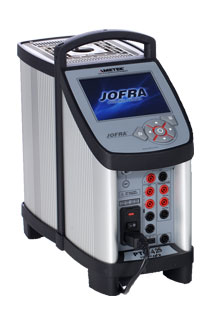
\includegraphics[width=0.25\linewidth,height=\textheight,keepaspectratio]{images/ametek.jpg}

}

\caption{\label{fig-AMETEK}AMETEK Jofra PTC-155.}

\end{figure}%

El instrumento mencionado se utilizó junto a cuatro termopares tipo T,
estableciendo cinco puntos de referencia de temperatura en el intervalo
de 10°C a 50°C.

Para cada punto de calibración, se esperó aproximadamente 5 minutos para
que el calibrador alcanzara y estabilizara la temperatura deseada. Una
vez estabilizada, se registraron los datos durante 10 minutos antes de
proceder al siguiente punto. Los resultados obtenidos en esta campaña se
pueden observar en la Figura~\ref{fig-termopares}.

\begin{figure}

\centering{

\begin{verbatim}
Unable to display output for mime type(s): text/html
\end{verbatim}

}

\caption{\label{fig-termopares}Rangos de temperatura utilizados para la
calibración de los termopares.}

\end{figure}%

\subsubsection{Temperatura radiante}\label{temperatura-radiante}

Para la medición de la temperatura radiante se empleó el QUESTemp 32
(Figura~\ref{fig-quest}), un confortímetro diseñado para evaluar el
estrés térmico en el ambiente, ya que permite medir la temperatura
radiante, la temperatura del aire y la humedad relativa.

\begin{figure}

\centering{

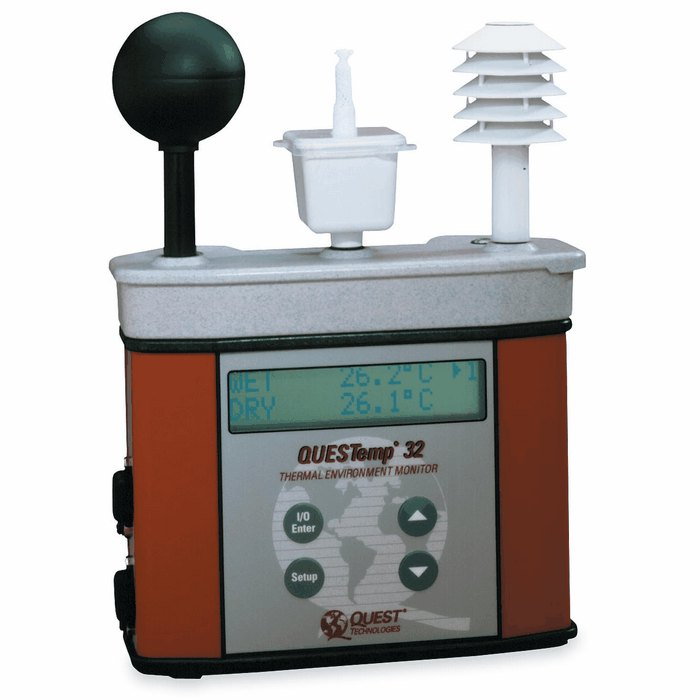
\includegraphics[width=0.3\linewidth,height=\textheight,keepaspectratio]{images/quest.jpeg}

}

\caption{\label{fig-quest}Quest Technologies QUESTemp 32.}

\end{figure}%

El experimento consistió en ubicar el QUESTemp 32 dentro de una caja
diseñada para limitar la incidencia directa de la radiación solar, lo
que minimizó la influencia de la radiación externa y redujo el efecto de
la convección forzada del viento, permitiendo así que la medición se
centrara en la radiación térmica del entorno inmediato. Paralelamente,
se colocó el sensor TPF1 en condiciones similares para garantizar que
ambos dispositivos registraran la temperatura con la menor perturbación
posible. Se tomaron datos cada minuto durante 23 horas. Los datos
obtenidos se pueden observar en la Figura~\ref{fig-radiante}.

\begin{figure}

\centering{

\begin{verbatim}
Unable to display output for mime type(s): text/html
\end{verbatim}

}

\caption{\label{fig-radiante}Intervalo de medición del QUESTemp 32 y el
TPF1 para su calibración.}

\end{figure}%

\subsubsection{Velocidad del viento}\label{velocidad-del-viento}

El WindMaster de Gill Instruments (Figura~\ref{fig-wind}) es un
anemómetro ultrasónico de alta precisión diseñado para medir la
velocidad y dirección del viento en tres direcciones (u, v, w). En esta
campaña se utilizó como instrumento de referencia para la calibración
del Wind Sensor.

\begin{figure}

\centering{

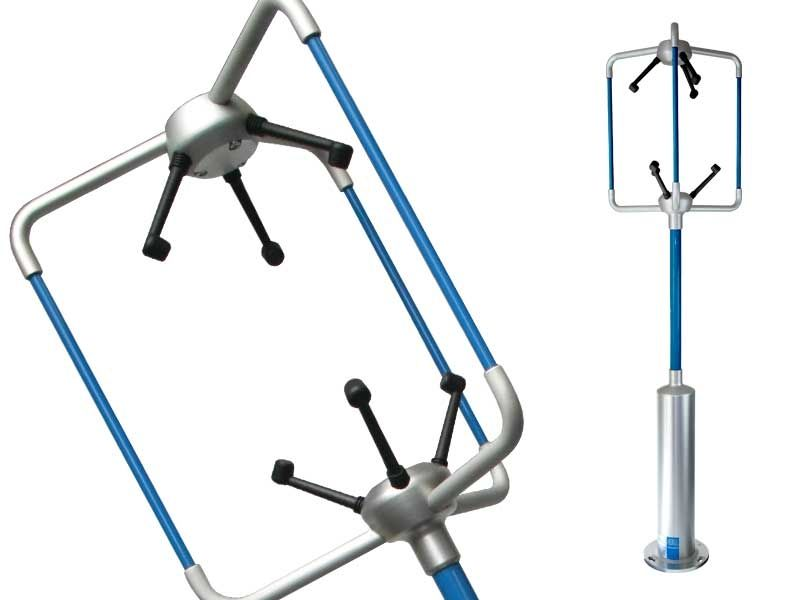
\includegraphics[width=0.35\linewidth,height=\textheight,keepaspectratio]{images/windmaster.jpg}

}

\caption{\label{fig-wind}Gill Instruments WindMaster.}

\end{figure}%

La campaña de calibración tuvo una duración de 1 hora, durante la cual
se capturaron datos a una frecuencia de 1 muestra por segundo.
Aprovechando las dimensiones del WindSensor (2230 x 680 mm), se
posicionó estratégicamente en la parte superior central del WindMaster,
previa verificación de que su presencia no interfiriera con las
mediciones del anemómetro. En un entorno abierto, el WindSensor registró
datos de voltaje, los cuales se utilizaron junto con los datos de
velocidad del viento obtenidos del WindMaster para desarrollar una
ecuación de calibración que permitiera convertir el voltaje medido a
m/s. Los resultados de la campaña se pueden visualizar en la
Figura~\ref{fig-viento}.

\begin{figure}

\centering{

\begin{verbatim}
Unable to display output for mime type(s): text/html
\end{verbatim}

}

\caption{\label{fig-viento}Comparación de la velocidad del viento
registrada por el WindMaster y el voltaje del Wind Sensor para su
calibración.}

\end{figure}%

\subsubsection{Humedad relativa y CO2}\label{humedad-relativa-y-co2}

Para la campaña de referenciación del SCD30, el instrumento utilizado
fue el Fluke 975 AirMeter (Figura~\ref{fig-fluke}), este es un
instrumento portátil de diagnóstico de la calidad del aire interior.
Este dispositivo mide simultáneamente temperatura, humedad relativa,
dióxido de carbono (CO2) y monóxido de carbono (CO).

\begin{figure}

\centering{

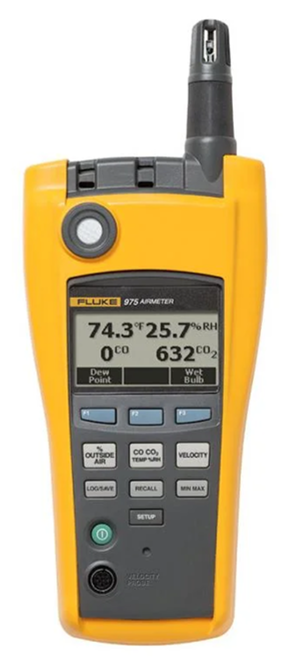
\includegraphics[width=0.15\linewidth,height=\textheight,keepaspectratio]{images/fluke.png}

}

\caption{\label{fig-fluke}Fluke 975 AirMeter.}

\end{figure}%

La campaña consistió en realizar mediciones simultáneas del Fluke 975
AirMeter y del SCD30 durante un período total de 7 horas y 45 minutos,
registrando una muestra cada minuto. Para minimizar posibles
interferencias, ambos dispositivos se ubicaron lo más próximos posible y
se instalaron en una zona aislada de un espacio cerrado, de modo que la
presencia humana no afectara los resultados. Los datos obtenidos se
muestran en la Figura~\ref{fig-calidad}.

\begin{figure}

\centering{

\begin{verbatim}
Unable to display output for mime type(s): text/html
\end{verbatim}

}

\caption{\label{fig-calidad}Comparación de las mediciones del Fluke y el
SCD30 durante su campaña de referenciación.}

\end{figure}%

\subsubsection{Sonido}\label{sonido}

\begin{figure}

\centering{

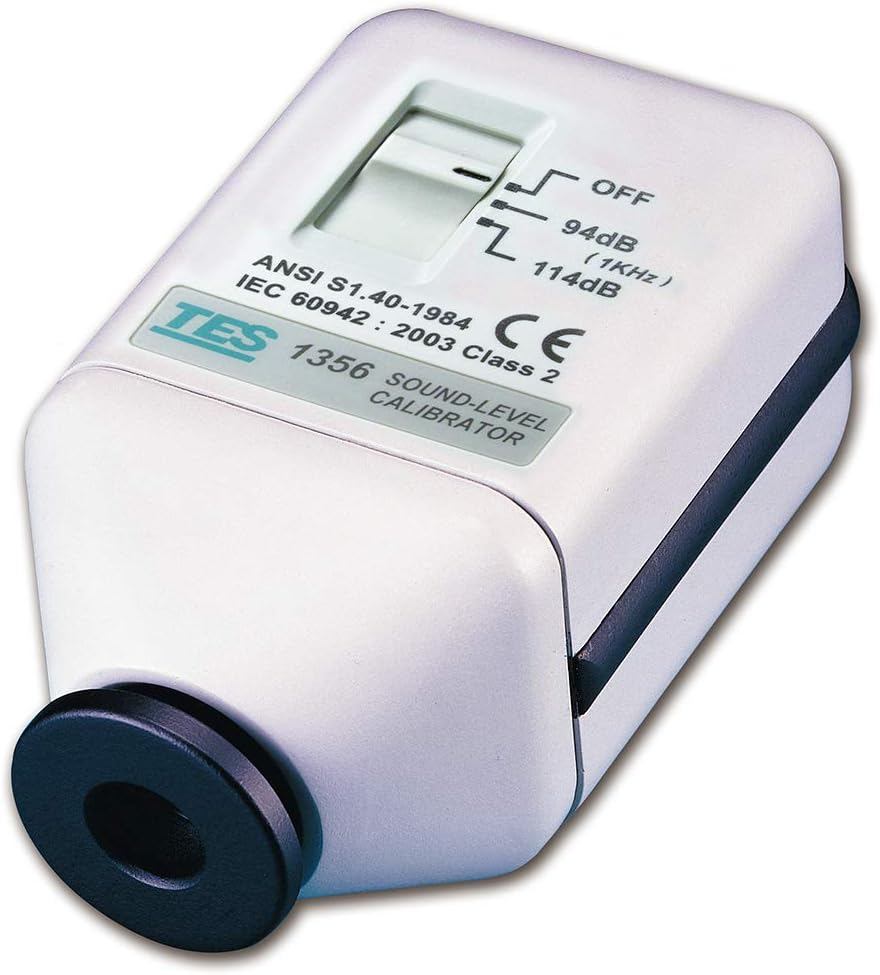
\includegraphics[width=0.2\linewidth,height=\textheight,keepaspectratio]{images/tes.jpg}

}

\caption{\label{fig-tes}TES-1356 Sound Level Calibrator.}

\end{figure}%

\section{Análisis e interpretación de
resultados}\label{anuxe1lisis-e-interpretaciuxf3n-de-resultados}

\subsubsection{Temperatura ambiente}\label{temperatura-ambiente-1}

\begin{figure}

\centering{

\begin{verbatim}
Unable to display output for mime type(s): text/html
\end{verbatim}

}

\caption{\label{fig-ctermopares}Resultados de las mediciones de
temperatura después de aplicar la ecuación de calibración.}

\end{figure}%

\subsubsection{Temperatura radiante}\label{temperatura-radiante-1}

\begin{figure}

\centering{

\begin{verbatim}
Unable to display output for mime type(s): text/html
\end{verbatim}

}

\caption{\label{fig-cradiante}Comparación de las mediciones del QUESTemp
32, el TPF1 y sus datos tras la calibración.}

\end{figure}%

\subsubsection{Velocidad del viento}\label{velocidad-del-viento-1}

\begin{figure}

\centering{

\begin{verbatim}
Unable to display output for mime type(s): text/html
\end{verbatim}

}

\caption{\label{fig-cviento}Comparación de las mediciones de velocidad
del viento registradas por el WindMaster y el Wind Sensor tras su
calibración.}

\end{figure}%

\subsubsection{Humedad relativa y CO2}\label{humedad-relativa-y-co2-1}

\begin{figure}

\centering{

\begin{verbatim}
Unable to display output for mime type(s): text/html
\end{verbatim}

}

\caption{\label{fig-ccalidad}Correlación de las mediciones de humedad
relativa, CO2 y temperatura entre el Fluke y el SCD30.}

\end{figure}%

\subsubsection{Sonido}\label{sonido-1}

\bookmarksetup{startatroot}

\chapter{Discusión y conclusiones}\label{discusiuxf3n-y-conclusiones}

\section{Trabajo a futuro}\label{trabajo-a-futuro}

\bookmarksetup{startatroot}

\chapter*{Bibliografía}\label{bibliografuxeda}
\addcontentsline{toc}{chapter}{Bibliografía}

\markboth{Bibliografía}{Bibliografía}

\phantomsection\label{refs}
\begin{CSLReferences}{1}{0}
\bibitem[\citeproctext]{ref-adafruit}
Adafruit. s.~f. {«Adafruit PT1000 RTD Temperature Sensor Amplifier -
MAX31865»}. \url{https://www.adafruit.com/product/3648\#description}.

\bibitem[\citeproctext]{ref-antoniadou}
Antoniadou, Panagiota, y Agis M. Papadopoulos. 2017. {«Occupants'
thermal comfort: State of the art and the prospects of personalized
assessment in office buildings»}. \emph{Energy and Buildings} 153:
136-49. \url{https://doi.org/10.1016/j.enbuild.2017.08.001}.

\bibitem[\citeproctext]{ref-arducam}
Arducam. s.~f. {«Arducam 5MP OV5647 Ultra Wide Angle Fisheye Camera for
Raspberry Pi»}.
\url{https://www.arducam.com/product/arducam-ultra-wide-angle-fisheye-5mp-ov5647-camera-for-raspberry-pi/}.

\bibitem[\citeproctext]{ref-arduino}
Arduino. 2023. {«Arduino UNO WiFi Rev2»}.
\url{https://store.arduino.cc/products/arduino-uno-wifi-rev2}.

\bibitem[\citeproctext]{ref-ashrae55}
ASHRAE-55. 2021. \emph{ANSI/ASHRAE Standard 55-2020: Thermal
Environmental Conditions for Human Occupancy}. Atlanta, GA: American
Society of Heating, Refrigerating; Air-Conditioning Engineers (ASHRAE).

\bibitem[\citeproctext]{ref-air}
ASHRAE-62. 2001. \emph{ANSI/ASHRAE Standard 62-2001: Ventilation for
acceptable indoor air quality}. Vol. 62. 2001. American Society of
Heating, Refrigerating; Air-Conditioning Engineers.

\bibitem[\citeproctext]{ref-azar}
Azar, Elie, William O'Brien, Salvatore Carlucci, Tianzhen Hong, Andrew
Sonta, Joyce Kim, Maedot S. Andargie, et~al. 2020. {«Simulation-aided
occupant-centric building design: A critical review of tools, methods,
and applications»}. \emph{Energy and Buildings} 224: 110292.
\url{https://doi.org/10.1016/j.enbuild.2020.110292}.

\bibitem[\citeproctext]{ref-berglund}
Berglund, B. 1999. {«Guidelines for community noise»}. \emph{World
Health Organization}.

\bibitem[\citeproctext]{ref-cie_illum}
CIE. 2020a. {«Illuminance (17-21-060)»}.
\url{https://cie.co.at/eilvterm/17-21-060}.

\bibitem[\citeproctext]{ref-cie_lum}
---------. 2020b. {«Luminance (17-21-050)»}.
\url{https://cie.co.at/eilvterm/17-21-050}.

\bibitem[\citeproctext]{ref-djongyang}
Djongyang, Noël, René Tchinda, y Donatien Njomo. 2010. {«Thermal
comfort: A review paper»}. \emph{Renewable and Sustainable Energy
Reviews} 14 (9): 2626-40.
\url{https://doi.org/10.1016/j.rser.2010.07.040}.

\bibitem[\citeproctext]{ref-fuehler}
FuehlerSysteme. s.~f. {«Radiation Pendulum Temperature Sensor»}.
\url{https://www.fuehlersysteme.de/Radiation-Pendulum-Temperature-Sensor_1\#70bd/embedded/}.

\bibitem[\citeproctext]{ref-macpherson}
Macpherson, R. K. 1962. {«The assessment of the thermal environment: A
review»}. \emph{British Journal of Industrial Medicine} 19 (3): 151-64.
\url{https://doi.org/10.1136/oem.19.3.151}.

\bibitem[\citeproctext]{ref-modern}
ModernDevice. s.~f. {«Wind Sensor Rev. P»}.
\url{https://moderndevice.com/products/wind-sensor-rev-p}.

\bibitem[\citeproctext]{ref-omega}
OMEGA. s.~f. {«¿Qué es un sensor termopar?»}
\url{https://es.omega.com/prodinfo/termopares.html\#}.

\bibitem[\citeproctext]{ref-pwf}
PWFusion. s.~f. {«4-Channel T-Type Thermocouple MAX31856 SPI Digital
Arduino Shield»}.
\url{https://www.playingwithfusion.com/productview.php?pdid=71&catid=1008}.

\bibitem[\citeproctext]{ref-raspberry}
Raspberry. 2019. {«Raspberry Pi 4 Model B»}.
\url{https://www.raspberrypi.com/products/raspberry-pi-4-model-b/}.

\bibitem[\citeproctext]{ref-scd30}
Sensirion. s.~f. {«SCD30»}.
\url{https://sensirion.com/products/catalog/SCD30}.

\bibitem[\citeproctext]{ref-light}
Standard, British. 2011. {«Light and lighting: Lighting of work places:
Part 1: Indoor work places»}. \emph{NS-EN 12464-1: 2011}.

\bibitem[\citeproctext]{ref-steren}
Steren. s.~f. {«Micrófono USB C de solapa para celular»}.
\url{https://www.steren.com.mx/microfono-usb-c-de-solapa-para-celular.html}.

\bibitem[\citeproctext]{ref-vasquez}
Vásquez, Natalia Giraldo, Maíra Longhinotti Felippe, Fernando O. R.
Pereira, y Ariane Kuhnen. 2019. {«Luminous and visual preferences of
young children in their classrooms: Curtain use, artificial lighting and
window views»}. \emph{Building and Environment} 152: 59-73.
\url{https://doi.org/10.1016/j.buildenv.2019.01.049}.

\end{CSLReferences}

\bookmarksetup{startatroot}

\chapter*{Anexos}\label{anexos}
\addcontentsline{toc}{chapter}{Anexos}

\markboth{Anexos}{Anexos}

This is a book created from markdown and executable code.


\backmatter


\end{document}
